\documentclass{article}
\usepackage{longtable}
\usepackage{array}
\usepackage{lscape}
\usepackage{graphicx}
\usepackage{hcmus-report-template}
\usepackage{tikz}  
% \usetikzlibrary{graphdrawing.trees}

\usetikzlibrary{arrows, positioning, shapes.multipart}
\usepackage{eso-pic}
\usetikzlibrary{calc,decorations.pathmorphing}
% Disable indentation on new paragraphs
\setlength{\parindent}{0pt}

% Line spacing 1.5
\renewcommand{\baselinestretch}{1.5}

% Optional: graphic path
% \graphicspath{PATH_TO_GRAPHIC_FOLDER}

% To use Times font family, uncomment this row
% \usepackage{mathptmx}

% To use roman section / subsection, uncomment these rows
% \renewcommand{\thesection}{\Roman{section}}
% \renewcommand{\thesubsection}{\thesection.\Roman{subsection}}

% Define course name, report name and report title.
\newcommand{\coursename}{Data Structures and Algorithms}
\newcommand{\reportname}{String Algorithms}
\newcommand{\reporttitle}{KMP and Aho-Corasick}

\newcommand{\studentname}{Võ Đình Cao Minh Hào (24127035)\\Trịnh Duy Nhân (24127094)\\Phan Thanh Trúc Quân (24127227)}
\newcommand{\teachername}{Dr. Nguyễn Ngọc Thảo \\ BSc. Nguyễn Thanh Tình}

% Header
\lhead{\reporttitle}
\rhead{
VNUHCM - University of Science\\
\coursename
}

% Footer
\newcommand{\leftfooter}{Report in \LaTeX\ by \href{https://github.com/HaoVoxx/Group-8-Course-Project}{Group 8}}
\lfoot{\leftfooter}

% ============ DOCUMENT ============
\begin{document}
\begin{titlepage}
  \AddToShipoutPictureBG*{%
    \begin{tikzpicture}[overlay,remember picture]
      \draw [line width=3pt]
        ($ (current page.north west) + (1.5cm,-2.0cm) $)
        rectangle
        ($ (current page.south east) + (-1.5cm,1.8cm) $);
      \draw [line width=1pt]
        ($ (current page.north west) + (1.65cm,-2.15cm) $)
        rectangle
        ($ (current page.south east) + (-1.65cm,1.95cm) $);
    \end{tikzpicture}%
  }
  \begin{center}
    \vspace*{\fill}
    \textsc{\LARGE VIETNAM NATIONAL UNIVERSITY \\ HO CHI MINH CITY}\\[0.5cm]
    \textsc{\LARGE UNIVERSITY OF SCIENCE}\\[0.5cm]
    \textsc{\Large FACULTY OF INFORMATION TECHNOLOGY}\\[1.0cm]
    \textsc{\LARGE DATA STRUCTURES AND ALGORITHMS}\\[0.5cm]
    \textsc{\LARGE KMP AND AHO-CORASICK}\\[1.5cm]
    
\includegraphics[width=5cm]{img/hcmus-logo.png}\\[1.5cm]
    \textsc{\large \bfseries Võ Đình Cao Minh Hào - 24127035}\\
    \textsc{\large \bfseries Trịnh Duy Nhân - 24127094}\\
    \textsc{\large \bfseries Phan Thanh Trúc Quân - 24127227}\\[1.0cm]
    \large \today
    \vspace*{\fill}
  \end{center}
\end{titlepage}
\pagenumbering{roman}
\begin{titlepage}
  \AddToShipoutPictureBG*{%
    \begin{tikzpicture}[overlay,remember picture]
      \draw [line width=3pt]
        ($ (current page.north west) + (1.5cm,-2.0cm) $)
        rectangle
        ($ (current page.south east) + (-1.5cm,1.8cm) $);
      \draw [line width=1pt]
        ($ (current page.north west) + (1.65cm,-2.15cm) $)
        rectangle
        ($ (current page.south east) + (-1.65cm,1.95cm) $);
    \end{tikzpicture}%
  }
  \begin{center}
    \vspace*{\fill}
    \textsc{\LARGE VIETNAM NATIONAL UNIVERSITY \\ HO CHI MINH CITY}\\[0.5cm]
    \textsc{\LARGE UNIVERSITY OF SCIENCE}\\[0.5cm]
    \textsc{\Large FACULTY OF INFORMATION TECHNOLOGY}\\[1.0cm]
    \textsc{\LARGE DATA STRUCTURES AND ALGORITHMS}\\[0.5cm]
    \textsc{\LARGE KMP AND AHO-CORASICK}\\[1.5cm]
    
\includegraphics[width=5cm]{img/hcmus-logo.png}\\[1.5cm]
    \textsc{\large \bfseries Võ Đình Cao Minh Hào - 24127035}\\
    \textsc{\large \bfseries Trịnh Duy Nhân - 24127094}\\
    \textsc{\large \bfseries Phan Thanh Trúc Quân - 24127227}\\[1.0cm]
    \large \today
    \vspace*{\fill}
  \end{center}
\end{titlepage}

\tableofcontents
\pagebreak

\pagenumbering{arabic}
\setcounter{page}{1}

\section{History and Applications of the Knuth-Morris-Pratt (KMP) Algorithm}
\subsection{History}
The Knuth-Morris-Pratt (KMP) algorithm was developed by Donald Knuth, Vaughan Pratt, and James H. Morris in 1970 and was officially published in 1977. The KMP algorithm provides an efficient method for locating a substring $W$ within a larger string $S$. Instead of re-examining previously matched characters upon encountering a mismatch, the KMP algorithm leverages information inherent in the pattern $W$ itself to determine the next position for comparison.

One of the key advantages of the KMP algorithm is its high efficiency. It operates with a time complexity of $O(n+m)$, where $n$ is the length of the text $S$ and $m$ is the length of the pattern $W$. Furthermore, by utilizing the Longest Prefix Suffix (LPS) table, the algorithm eliminates redundant comparisons, thereby optimizing search performance. The KMP algorithm represents a significant improvement over conventional brute-force search methods, making it particularly beneficial when processing large datasets or executing repeated search operations.

\subsection{Applications}
\begin{itemize}
    \item Text searching: Implemented in text editors (such as Microsoft Word, Notepad++) to locate words or phrases within documents.
    \item Pattern matching in DNA and computational biology: Applied in genetic research to identify specific gene sequences within extensive DNA datasets.
    \item Spam filtering: Used to detect suspicious keywords in emails, aiding in the identification of spam messages.
    \item Search engines: Enhances search efficiency by facilitating substring searches within large-scale databases.
    \item Plagiarism detection: Compares textual documents to identify duplicated content, assisting in academic integrity verification.
    \item File processing and compilation: Employed in certain compilers to efficiently analyze and parse source code.
\end{itemize}
\section{Knuth - Morris - Pratt Step by step}
\textbf{Note}: The string will start at number 0

\subsection{Problem}
\begin{itemize}
    \item Given string s: "ABXABABABAA".
    \item Given string t: "ABABAA".
\end{itemize}

Check if string t exists in string s?

\subsection{Main idea}

The idea behind KMP is to extend a suffix ending at position i to a suffix ending at position i+1 while still matching the corresponding prefix, which improves efficiency by eliminating expensive string comparisons. \cite{vnoi}


\subsection{Definition}
\begin{itemize}
    \item \textbf{Proper Prefix}: A prefix that is not equal to the string itself.

    \item \textbf{Prefix Function}\cite{cpAlgo}: An array $\pi$ of length m, where $\pi[i]$ is the length of the longest proper prefix of the substring $s[0..i]$, which is also a suffix of the substring. Mathematically, the definition of the prefix function can be written as follows:
\end{itemize}
\begin{equation}
    \pi[i] = \max_{0 \le k \le i} \{\,k : s[0 \dots k-1] = s[i-(k-1) \dots i]\}.
\end{equation}

\subsection{Preprocessing}
Due to the definition of proper prefix, $\pi[0] = 0$.

Here is the example code:
\lstinputlisting[language=C++]{code/Preprocessing.cpp}
The example code will run in $\Theta(m)$ where m is the length of the pattern.
    \subsection *{Explain step by step}
    \textbf{Step 1: }$\pi[0] = 0$ so $i$ starts at 1. We use $j$ to trace the prefix, and it starts at 0:

    \begin{table}[H]
    \centering
    \begin{tabular}{|c|c|c|c|c|c|c|}
    \hline
    pos   & j & i &   &   &   &   \\ \hline
    t     & A & B & A & B & A & A \\ \hline
    $\pi$ & 0 &   &   &   &   &   \\ \hline
    \end{tabular}
    \end{table}
    
    \textbf{Step 2: }\textit{At $i = 1$ and $j = 0$}
    
    $t[i]$ mismatches $t[j]$ ("A" $\neq$ "B"), so we set $\pi[i = 1] = 0$ then increases $i$ by 1:
    \begin{table}[H]
    \centering
    \begin{tabular}{|c|c|c|c|c|c|c|}
    \hline
    pos   & $j$ &   & $i$ &   &   &   \\ \hline
    t     & A & B & A & B & A & A \\ \hline
    $\pi$ & 0 & 0 &   &   &   &   \\ \hline
    \end{tabular}
    \end{table}

    \textbf{Step 3: }\textit{At $i = 2$ and $j = 0$}
    
    $t[i]$ matches $t[j]$ ("A" $=$ "A"), so we set $\pi[i = 2] = j + 1 = 1$ then increases both $i$ and $j$ by 1:
    \begin{table}[H]
    \centering
    \begin{tabular}{|c|c|c|c|c|c|c|}
    \hline
    pos   &   & $j$ &   & $i$ &   &   \\ \hline
    t     & A & B & A & B & A & A \\ \hline
    $\pi$ & 0 & 0 & 1 &   &   &   \\ \hline
    \end{tabular}
    \end{table}
    \textbf{Note}: $\pi[i] = j + 1$ because $\pi[i]$ represents the length of the longest proper prefix of the substring $t[0\dots i]$, which is also a suffix of the substring.
    
    \textbf{Step 4: }\textit{At $i = 3$ and $j = 1$}
    
    $t[i]$ matches $t[j]$ ("B" $=$ "B"), so we set $\pi[i = 3] = j + 1 = 2$ then increases both $i$ and $j$ by 1:
    \begin{table}[H]
    \centering
    \begin{tabular}{|c|c|c|c|c|c|c|}
    \hline
    pos   &   &   & $j$ &   & $i$ &   \\ \hline
    t     & A & B & A & B & A & A \\ \hline
    $\pi$ & 0 & 0 & 1 & 2 &   &   \\ \hline
    \end{tabular}
    \end{table}
    \textbf{Step 5: }\textit{At $i = 4$ and $j = 2$}
    
    $t[i]$ matches $t[j]$ ("A" $=$ "A"), so we set $\pi[i = 4] = j + 1 = 3$ then increases both $i$ and $j$ by 1:
    \begin{table}[H]
    \centering
    \begin{tabular}{|c|c|c|c|c|c|c|}
    \hline
    pos   &   &   &   & $j$ &   & $i$ \\ \hline
    t     & A & B & A & B & A & A \\ \hline
    $\pi$ & 0 & 0 & 1 & 2 & 3 &   \\ \hline
    \end{tabular}
    \end{table}
    \textbf{Step 6: }\textit{At $i = 5$ and $j = 3$} 
    
    $t[i]$ mismatches $t[j]$ ("B" $\neq$ "A") and j is greater than 0. This situation is a bit tricky because we must trace back to the $\pi[j - 1]$ position. Since $\pi[i]$ represents the longest proper prefix of $s[0\dots i]$, $\pi[i - 1]$ represents the second longest proper prefix and so on. Therefore, if there is a mismatch, we have to trace back to the second, third, etc., longest proper prefix. In this case, $j$ moves to position 1 because $\pi[j - 1] = 1$:
    \begin{table}[H]
    \centering
    \begin{tabular}{|c|c|c|c|c|c|c|}
    \hline
    pos   &   & $j$ &   &   &   & $i$ \\ \hline
    t     & A & B & A & B & A & A \\ \hline
    $\pi$ & 0 & 0 & 1 & 2 & 3 &   \\ \hline
    \end{tabular}
    \end{table}
    \textbf{Step 7: }Now, $t[i]$ and $t[j]$ still do not match, and $j$ is still greater than 0, so we repeat the backtracking step. As a result, $j$ goes back to $0$ because $\pi[j - 1] = 0$:
    \begin{table}[H]
    \centering
    \begin{tabular}{|c|c|c|c|c|c|c|}
    \hline
    pos   & $j$ &   &   &   &   & $i$ \\ \hline
    t     & A & B & A & B & A & A \\ \hline
    $\pi$ & 0 & 0 & 1 & 2 & 3 &   \\ \hline
    \end{tabular}
    \end{table}
    \textbf{Step 8: }Now, $t[i]$ and $t[j]$ match ("A" $=$ "A") so we set $\pi[i] = j + 1 = 1$ and done the prefix function.
    \begin{table}[H]
    \centering
    \begin{tabular}{|c|c|c|c|c|c|c|}
    \hline
    t     & A & B & A & B & A & A \\ \hline
    $\pi$ & 0 & 0 & 1 & 2 & 3 & 1 \\ \hline
    \end{tabular}
    \end{table}

    \textbf{Important}: The code always runs in linear time regardless of the string's distribution. Therefore, the time and space complexity of the code is $\Theta(m)$, where m is the length of the pattern string.
\subsection{String matching}

After computing the prefix function for the pattern \( t \), we use it to efficiently search for \( t \) in the text \( s \). Recall that for \( t = \texttt{ABABAA} \), the prefix function is:
\[
\pi = [0,\, 0,\, 1,\, 2,\, 3,\, 1].
\]

The string matching algorithm proceeds as follows:

\begin{enumerate}
    \item Initialize two indices: \( i \) for the text \( s \) (starting at 0) and \( j \) for the pattern \( t \) (starting at 0).
    \item Compare \( s[i] \) with \( t[j] \):
    \begin{itemize}
        \item If \( s[i] = t[j] \), increment both \( i \) and \( j \).
        \item If \( s[i] \neq t[j] \) and \( j > 0 \), update \( j \) to \( \pi[j-1] \) (i.e., backtrack \( j \) to the length of the next best candidate prefix) and compare again.
        \item If \( s[i] \neq t[j] \) and \( j = 0 \), increment \( i \) only.
    \end{itemize}
    \item If \( j \) reaches the length of \( t \) (i.e., \( j = m \) where \( m \) is the length of \( t \)), a full match is found at index \( i - j \) in \( s \).
\end{enumerate}

\subsection*{Example Walk-through}
Consider the given strings:
\begin{itemize}
    \item \( s = \texttt{ABXABABABAA} \)
    \item \( t = \texttt{ABABAA} \)
\end{itemize}
\textbf{Step 1: }\textit{Start with i = 0 and j = 0}

\begin{table}[H]
\centering
\begin{tabular}{|c|c|c|c|c|c|c|c|c|c|c|c|}
\hline
pos   &$i$&   &   &   &   &   &   &   &   &   &   \\ \hline
s     & A & B & X & A & B & A & B & A & B & A & A \\ \hline
\end{tabular}
\end{table}

\begin{table}[H]
\centering
\begin{tabular}{|c|c|c|c|c|c|c|}
\hline
pos   & $j$ &   &   &   &   &   \\ \hline
t     & A & B & A & B & A & A \\ \hline
$\pi$ & 0 & 0 & 1 & 2 & 3 & 1 \\ \hline
\end{tabular}
\end{table}

$s[0] = $ \texttt{A} and $t[0] = $ \texttt{A} $\longrightarrow$ match, so increment: $i = 1$, $j = 1$.

\textbf{Step 2: }\textit{Now, $i = 1$ and $j = 1$}

\begin{table}[H]
\centering
\begin{tabular}{|c|c|c|c|c|c|c|c|c|c|c|c|}
\hline
pos   &   &$i$&   &   &   &   &   &   &   &   &   \\ \hline
s     & A & B & X & A & B & A & B & A & B & A & A \\ \hline
\end{tabular}
\end{table}

\begin{table}[H]
\centering
\begin{tabular}{|c|c|c|c|c|c|c|}
\hline
pos   &   & $j$ &   &   &   &   \\ \hline
t     & A & B & A & B & A & A \\ \hline
$\pi$ & 0 & 0 & 1 & 2 & 3 & 1 \\ \hline
\end{tabular}
\end{table}

$s[1] = $ \texttt{B} and $t[1] = $ \texttt{B} $\longrightarrow$ match, so increment: $i = 2$, $j = 2$.

\textbf{Step 3: }\textit{Now, $i = 2$ and $j = 2$}

\begin{table}[H]
\centering
\begin{tabular}{|c|c|c|c|c|c|c|c|c|c|c|c|}
\hline
pos   &   &   &$i$&   &   &   &   &   &   &   &   \\ \hline
s     & A & B & X & A & B & A & B & A & B & A & A \\ \hline
\end{tabular}
\end{table}

\begin{table}[H]
\centering
\begin{tabular}{|c|c|c|c|c|c|c|}
\hline
pos   &   &   & $j$ &   &   &   \\ \hline
t     & A & B & A & B & A & A \\ \hline
$\pi$ & 0 & 0 & 1 & 2 & 3 & 1 \\ \hline
\end{tabular}
\end{table}

$s[2] = $ \texttt{X} and $t[2] = $ \texttt{A} $\longrightarrow$ mismatch.

Since $j > 0$, update $j$ to $\pi[j - 1] = \pi[1] = 0$.

\textbf{Step 4: }\textit{Now, $i = 2$ and $j = 0$}

\begin{table}[H]
\centering
\begin{tabular}{|c|c|c|c|c|c|c|c|c|c|c|c|}
\hline
pos   &   &   &$i$&   &   &   &   &   &   &   &   \\ \hline
s     & A & B & X & A & B & A & B & A & B & A & A \\ \hline
\end{tabular}
\end{table}

\begin{table}[H]
\centering
\begin{tabular}{|c|c|c|c|c|c|c|}
\hline
pos   & $j$ &   &   &   &   &   \\ \hline
t     & A & B & A & B & A & A \\ \hline
$\pi$ & 0 & 0 & 1 & 2 & 3 & 1 \\ \hline
\end{tabular}
\end{table}

$s[2] = $ \texttt{X} and $t[0] = $ \texttt{A} $\longrightarrow$ mismatch.

But now $j = 0$, so increment: $i = 3$.

\textbf{Step 5: }\textit{Now, $i = 3$ and $j = 0$}

\begin{table}[H]
\centering
\begin{tabular}{|c|c|c|c|c|c|c|c|c|c|c|c|}
\hline
pos   &   &   &   &$i$&   &   &   &   &   &   &   \\ \hline
s     & A & B & X & A & B & A & B & A & B & A & A \\ \hline
\end{tabular}
\end{table}

\begin{table}[H]
\centering
\begin{tabular}{|c|c|c|c|c|c|c|}
\hline
pos   & $j$ &   &   &   &   &   \\ \hline
t     & A & B & A & B & A & A \\ \hline
$\pi$ & 0 & 0 & 1 & 2 & 3 & 1 \\ \hline
\end{tabular}
\end{table}

$s[3] = $ \texttt{A} and $t[0] = $ \texttt{A} $\longrightarrow$ match, so increment: $i = 4$, $j = 1$.

\textbf{Step 6: }\textit{Now, $i = 4$ and $j = 1$}

\begin{table}[H]
\centering
\begin{tabular}{|c|c|c|c|c|c|c|c|c|c|c|c|}
\hline
pos   &   &   &   &   &$i$&   &   &   &   &   &   \\ \hline
s     & A & B & X & A & B & A & B & A & B & A & A \\ \hline
\end{tabular}
\end{table}

\begin{table}[H]
\centering
\begin{tabular}{|c|c|c|c|c|c|c|}
\hline
pos   &   & $j$ &   &   &   &   \\ \hline
t     & A & B & A & B & A & A \\ \hline
$\pi$ & 0 & 0 & 1 & 2 & 3 & 1 \\ \hline
\end{tabular}
\end{table}

$s[4] = $ \texttt{B} and $t[1] = $ \texttt{B} $\longrightarrow$ match, so increment: $i = 5$, $j = 2$.

\textbf{Step 7: }\textit{Now, $i = 5$ and $j = 2$}

\begin{table}[H]
\centering
\begin{tabular}{|c|c|c|c|c|c|c|c|c|c|c|c|}
\hline
pos   &   &   &   &   &   &$i$&   &   &   &   &   \\ \hline
s     & A & B & X & A & B & A & B & A & B & A & A \\ \hline
\end{tabular}
\end{table}

\begin{table}[H]
\centering
\begin{tabular}{|c|c|c|c|c|c|c|}
\hline
pos   &   &   &$j$&   &   &   \\ \hline
t     & A & B & A & B & A & A \\ \hline
$\pi$ & 0 & 0 & 1 & 2 & 3 & 1 \\ \hline
\end{tabular}
\end{table}

$s[5] = $ \texttt{A} and $t[2] = $ \texttt{A} $\longrightarrow$ match, so increment: $i = 6$, $j = 3$.

\textbf{Step 8: }\textit{Now, $i = 6$ and $j = 3$}

\begin{table}[H]
\centering
\begin{tabular}{|c|c|c|c|c|c|c|c|c|c|c|c|}
\hline
pos   &   &   &   &   &   &   &$i$&   &   &   &   \\ \hline
s     & A & B & X & A & B & A & B & A & B & A & A \\ \hline
\end{tabular}
\end{table}

\begin{table}[H]
\centering
\begin{tabular}{|c|c|c|c|c|c|c|}
\hline
pos   &   &   &   &$j$&   &   \\ \hline
t     & A & B & A & B & A & A \\ \hline
$\pi$ & 0 & 0 & 1 & 2 & 3 & 1 \\ \hline
\end{tabular}
\end{table}

$s[6] = $ \texttt{B} and $t[3] = $ \texttt{B} $\longrightarrow$ match, so increment: $i = 7$, $j = 4$.

\textbf{Step 9: }\textit{Now, $i = 7$ and $j = 4$}

\begin{table}[H]
\centering
\begin{tabular}{|c|c|c|c|c|c|c|c|c|c|c|c|}
\hline
pos   &   &   &   &   &   &   &   &$i$&   &   &   \\ \hline
s     & A & B & X & A & B & A & B & A & B & A & A \\ \hline
\end{tabular}
\end{table}

\begin{table}[H]
\centering
\begin{tabular}{|c|c|c|c|c|c|c|}
\hline
pos   &   &   &   &   &$j$&   \\ \hline
t     & A & B & A & B & A & A \\ \hline
$\pi$ & 0 & 0 & 1 & 2 & 3 & 1 \\ \hline
\end{tabular}
\end{table}

$s[7] = $ \texttt{A} and $t[4] = $ \texttt{A} $\longrightarrow$ match, so increment: $i = 8$, $j = 5$.

\textbf{Step 10: }\textit{Now, $i = 8$ and $j = 5$}

\begin{table}[H]
\centering
\begin{tabular}{|c|c|c|c|c|c|c|c|c|c|c|c|}
\hline
pos   &   &   &   &   &   &   &   &   &$i$&   &   \\ \hline
s     & A & B & X & A & B & A & B & A & B & A & A \\ \hline
\end{tabular}
\end{table}

\begin{table}[H]
\centering
\begin{tabular}{|c|c|c|c|c|c|c|}
\hline
pos   &   &   &   &   &   &$j$\\ \hline
t     & A & B & A & B & A & A \\ \hline
$\pi$ & 0 & 0 & 1 & 2 & 3 & 1 \\ \hline
\end{tabular}
\end{table}

$s[8] = $ \texttt{B} and $t[5] = $ \texttt{A} $\longrightarrow$ mismatch.

Since $j > 0$, update $j$ to $\pi[j - 1] = \pi[4] = 3$.

\textbf{Step 11: }\textit{Now, $i = 8$ and $j = 3$}

\begin{table}[H]
\centering
\begin{tabular}{|c|c|c|c|c|c|c|c|c|c|c|c|}
\hline
pos   &   &   &   &   &   &   &   &   &$i$&   &   \\ \hline
s     & A & B & X & A & B & A & B & A & B & A & A \\ \hline
\end{tabular}
\end{table}

\begin{table}[H]
\centering
\begin{tabular}{|c|c|c|c|c|c|c|}
\hline
pos   &   &   &   &$j$&   &   \\ \hline
t     & A & B & A & B & A & A \\ \hline
$\pi$ & 0 & 0 & 1 & 2 & 3 & 1 \\ \hline
\end{tabular}
\end{table}

$s[8] = $ \texttt{B} and $t[3] = $ \texttt{B} $\longrightarrow$ match, so increment: $i = 9$, $j = 4$.

\textbf{Step 12: }\textit{Now, $i = 9$ and $j = 4$}

\begin{table}[H]
\centering
\begin{tabular}{|c|c|c|c|c|c|c|c|c|c|c|c|}
\hline
pos   &   &   &   &   &   &   &   &   &   &$i$&   \\ \hline
s     & A & B & X & A & B & A & B & A & B & A & A \\ \hline
\end{tabular}
\end{table}

\begin{table}[H]
\centering
\begin{tabular}{|c|c|c|c|c|c|c|}
\hline
pos   &   &   &   &   &$j$&   \\ \hline
t     & A & B & A & B & A & A \\ \hline
$\pi$ & 0 & 0 & 1 & 2 & 3 & 1 \\ \hline
\end{tabular}
\end{table}

$s[9] = $ \texttt{A} and $t[4] = $ \texttt{A} $\longrightarrow$ match, so increment: $i = 10$, $j = 5$.

\textbf{Step 13: }\textit{Now, $i = 10$ and $j = 5$}

\begin{table}[H]
\centering
\begin{tabular}{|c|c|c|c|c|c|c|c|c|c|c|c|}
\hline
pos   &   &   &   &   &   &   &   &   &   &   &$i$\\ \hline
s     & A & B & X & A & B & A & B & A & B & A & A \\ \hline
\end{tabular}
\end{table}

\begin{table}[H]
\centering
\begin{tabular}{|c|c|c|c|c|c|c|}
\hline
pos   &   &   &   &   &   &$j$\\ \hline
t     & A & B & A & B & A & A \\ \hline
$\pi$ & 0 & 0 & 1 & 2 & 3 & 1 \\ \hline
\end{tabular}
\end{table}

$s[10] = $ \texttt{A} and $t[5] = $ \texttt{A} $\longrightarrow$ match.

Since $j = m$ where m is the length of t, a full match is found at index $i - j = 5^{th}$ in $s$.

Here is the full code of String Matching:
\lstinputlisting[language=C++]{code/StringMatching.cpp}

The overall complexity of this string matching process is \( \mathcal{O}(n + m) \), where \( n \) is the length of the text \( s \) and \( m \) is the length of the pattern \( t \).

\subsection{Complexity Analysis}
\begin{itemize}
    \item The total \textbf{Space Complexity} of the algorithm is $\Theta(m)$, due to the contruction of $\pi$ length m.
    \item However, the \textbf{Time Complexity} of the algorithm depends on the kind of problem:
    \begin{itemize}
        \item Find all the position that string pattern $t$ occurs in string text $s$.
        \item Return the first string pattern $t$ occurs in string text $s$ or Check if string pattern $t$ occurs in string text or not.
    \end{itemize}
\end{itemize}
\subsection*{Find all the position}
\begin{itemize}
    \item In this problem, we must agree that the \textbf{Preprocessing} step always runs in $\Theta(m)$ because it always iterates through pattern $t$.
    \item In \textbf{String Matching} step, we also iterate through string $s$ to find all the position that appears pattern $t$. So the time complexity is $\Theta(n)$.
\end{itemize}
$\Longrightarrow$ The total \textbf{Time Complexity} is $\Theta(n + m)$
\subsection*{Check if occurs or not}
\begin{itemize}
    \item In this problem, we must agree that the \textbf{Preprocessing} step always runs in $\Theta(m)$ because it always iterates through pattern $t$.
    \item In \textbf{String Matching} step, it happens 2 cases:
    \begin{itemize}
        \item \textbf{Best Case:} We instantly find the pattern $t$ at the prefix of the string $s$.
        \item \textbf{Worst Case:} We find the pattern $t$ at the suffix of the string $s$.
    \end{itemize}
\end{itemize}
$\Longrightarrow$ The \textbf{Time Complexity} of the algorithm is:
\begin{itemize}
    \item \textbf{Best Case:} $\mathcal{O}(m)$.
    \item \textbf{Worst Case: } $\mathcal{O}(n + m)$.
\end{itemize}

\section{History and Applications of the Aho-Corasick Algorithm}
\subsection{History}
The Aho-Corasick algorithm was developed by Alfred V. Aho and Margaret J. Corasick in 1975. It is a multi-pattern string-searching algorithm that operates based on the Trie data structure, augmented with a failure function to enable efficient identification of multiple pattern occurrences within a given text. By constructing a finite-state automaton, the algorithm is capable of detecting multiple patterns concurrently in a single pass over the input text.

One of the primary advantages of the Aho-Corasick algorithm is its ability to search for multiple patterns simultaneously, eliminating the need for separate executions as required by algorithms such as KMP or Boyer-Moore. It achieves a time complexity of $O(n+m+z)$, where $n$ is the length of the input text, $m$ is the total length of all patterns, and $z$ is the number of pattern matches found. Additionally, the algorithm does not require redundant character comparisons, as the failure function enables efficient transitions upon mismatches. The Aho-Corasick algorithm finds extensive applications in network security, natural language processing, and computational biology. Due to its capability of handling large-scale multi-pattern searches, it significantly reduces processing time and resource consumption.

\subsection{Applications}
\begin{itemize}
    \item Network security and malware detection: Deployed in Intrusion Detection Systems (IDS) to identify attack signatures embedded within network traffic. Implemented in antivirus software to detect malware patterns within system files and memory.
    \item Text processing and keyword searching: Efficiently searches for multiple keywords simultaneously, making it ideal for content filtering in document processing, social media platforms, and email monitoring systems.
    \item Computational biology (bioinformatics): Utilized in DNA sequence analysis to locate multiple genetic markers or protein sequences within large genomic datasets, facilitating research in genetics and medicine.
    \item Spell checking and word suggestions: Applied in Natural Language Processing (NLP) to enhance spell checking and autocomplete functionalities, improving text input efficiency in word processing applications.
\end{itemize}


\section{Aho - Corasick Step by step}

\subsection{Problem}
Given the text: "DIDUDUADI".

Given the 6 patterns: "DI", "DIDU", "DIDI", "DU", "DUDUA", "DUADI".

Count how many patterns are there occur in the text?

\subsection{Main idea\cite{stanford}}
Aho-Corsick has 2 steps:

Step 1: Preprocessing process: Aho-Corasick uses trie structure to contain multiple patterns. In this trie structure, every node has a suffix link. At node i, the suffix link points to a node satisfies that prefix ends at that node is the longest suffix of string ending at node i.

Step 2: Searching/ Matching process: Aho-Corasick uses suffix link to link to the prefix when the mismatching occurs, so that we don’t have to check the same substring many times.
\subsection{Preprocessing\cite{vnoj}\cite{CpAlgor}}
There are two substeps in this process:

Step 1: Initialize a trie with suffix link pointing to the root to contain patterns.

Step 2: Linking the suffix link of each node to the node that satisfies the condition.

\subsubsection*{Initialize the trie with suffix link points to the root}
\pagebreak
\subsubsection*{Source code}
\lstinputlisting[language=C++]{code/initialize.cpp}
\subsubsection*{Result}
\begin{center}
    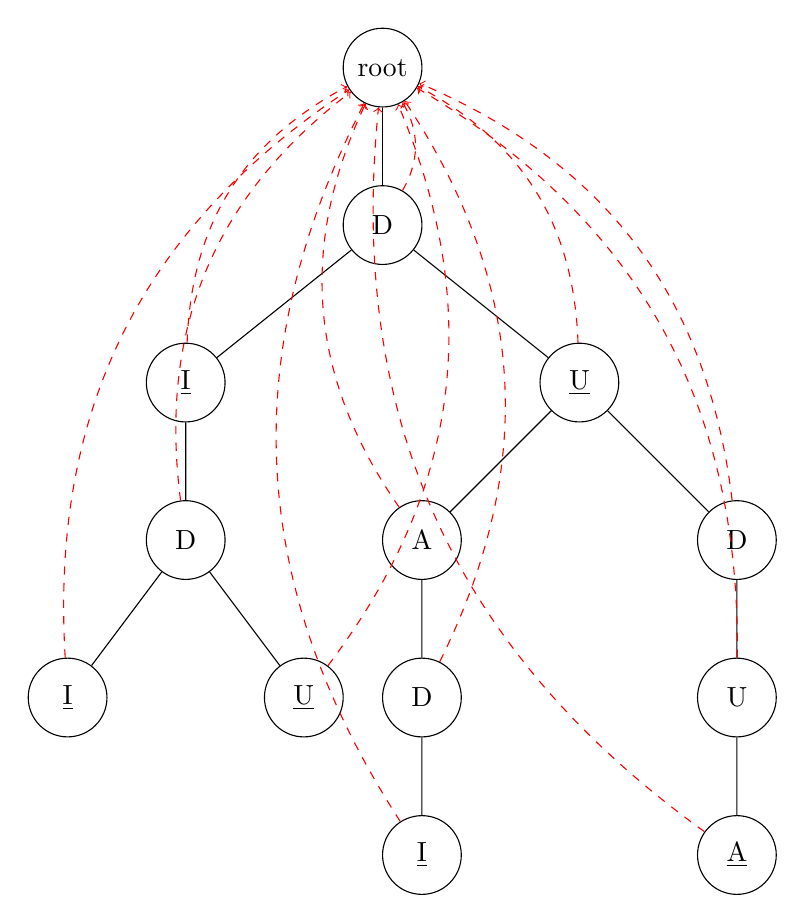
\begin{tikzpicture}[
        level 1/.style={sibling distance=6cm, level distance=2cm},
        level 2/.style={sibling distance=5cm, level distance=2cm},
        level 3/.style={sibling distance=4cm, level distance=2cm},
        level 4/.style={sibling distance=3cm, level distance=2cm},
        level 5/.style={sibling distance=2cm, level distance=2cm},
        level 6/.style={sibling distance=2cm, level distance=2ccm},
        every node/.style={circle, draw, minimum size=1cm}
    ]
        % Vẽ cây chính
        \node (root) {root}
            child { node (D1) {D}
                child { node (I) {\underline{I}}
                    child { node (D2) {D}
                        child { node (I2) {\underline{I} }}
                        child { node (U2) {\underline{U} }}
                    }
                }
                child { node (U1) {\underline{U}}
                    child { node (A2) {A}
                        child { node (D4) {D}
                            child { node (I3) {\underline{I} } }
                        }
                    }
                    child { node (D3) {D}
                        child { node (U3) {U}
                            child { node (A) {\underline{A} } }
                        }
                    }
                }
            };

        % Thêm các liên kết về gốc
        \draw[red, dashed, ->] (D1) to[bend right] (root);
        \draw[red, dashed, ->] (I) to[bend left] (root);
        \draw[red, dashed, ->] (I2) to[bend left] (root);
        \draw[red, dashed, ->] (D2) to[bend left] (root);
        \draw[red, dashed, ->] (U1) to[bend right] (root);
        \draw[red, dashed, ->] (D3) to[bend right] (root);
        \draw[red, dashed, ->] (U2) to[bend right] (root);
        \draw[red, dashed, ->] (A) to[bend left] (root);
        \draw[red, dashed, ->] (A2) to[bend left] (root);
        \draw[red, dashed, ->] (D4) to[bend right] (root);
        \draw[red, dashed, ->] (I3) to[bend left] (root);
        \draw[red, dashed, ->] (U3) to[bend right] (root);
    \end{tikzpicture}
\end{center}
\pagebreak
\subsection*{Linking the suffix link}
\subsubsection*{Source code}
\lstinputlisting[language=C++]{code/linking.cpp}
\pagebreak
\subsubsection*{Step by step}
\textbf{Step 1:}
\begin{center}
    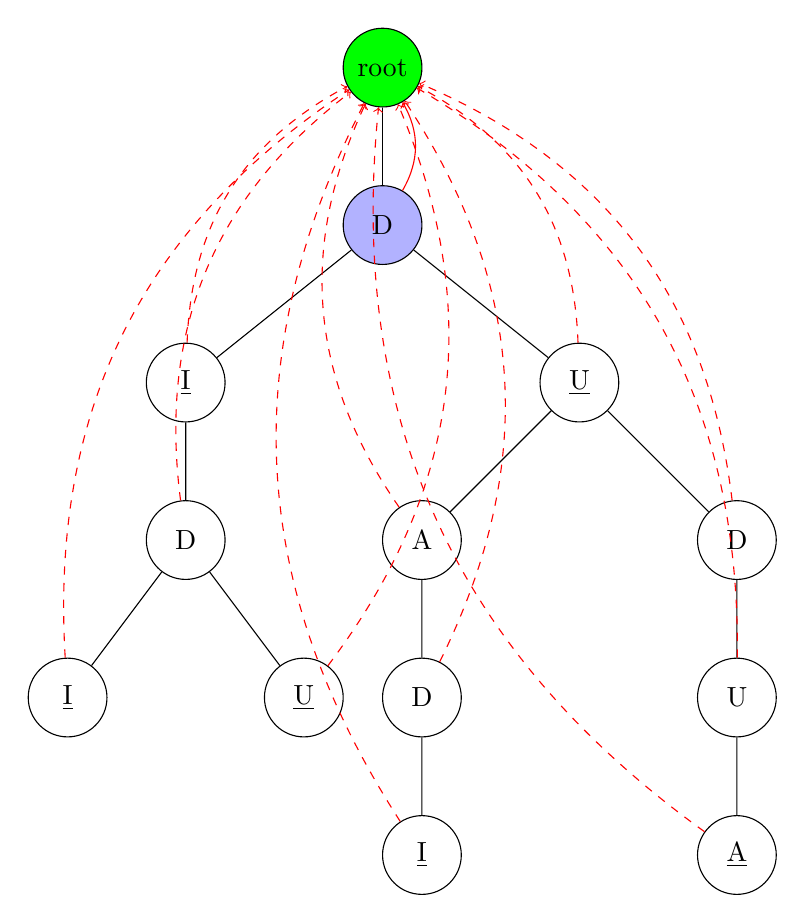
\begin{tikzpicture}[
        level 1/.style={sibling distance=6cm, level distance=2cm},
        level 2/.style={sibling distance=5cm, level distance=2cm},
        level 3/.style={sibling distance=4cm, level distance=2cm},
        level 4/.style={sibling distance=3cm, level distance=2cm},
        level 5/.style={sibling distance=2cm, level distance=2cm},
        level 6/.style={sibling distance=2cm, level distance=2ccm},
        every node/.style={circle, draw, minimum size=1cm}
    ]
        % Vẽ cây chính
        \node [fill=green](root) {root}
            child { node[fill=blue!30] (D1) {D}
                child { node (I) {\underline{I}}
                    child { node (D2) {D}
                        child { node (I2) {\underline{I}} }
                        child { node (U2) {\underline{U}} }
                    }
                }
                child { node (U1) {\underline{U}}
                    child { node (A2) {A}
                        child { node (D4) {D}
                            child { node (I3) {\underline{I}} }
                        }
                    }
                    child { node (D3) {D}
                        child { node (U3) {U}
                            child { node (A) {\underline{A}} }
                        }
                    }
                }
            };

        % Thêm các liên kết về gốc
        \draw[red, ->] (D1) to[bend right] (root);
        \draw[red, dashed, ->] (I) to[bend left] (root);
        \draw[red, dashed, ->] (I2) to[bend left] (root);
        \draw[red, dashed, ->] (D2) to[bend left] (root);
        \draw[red, dashed, ->] (U1) to[bend right] (root);
        \draw[red, dashed, ->] (D3) to[bend right] (root);
        \draw[red, dashed, ->] (U2) to[bend right] (root);
        \draw[red, dashed, ->] (A) to[bend left] (root);
        \draw[red, dashed, ->] (A2) to[bend left] (root);
        \draw[red, dashed, ->] (D4) to[bend right] (root);
        \draw[red, dashed, ->] (I3) to[bend left] (root);
        \draw[red, dashed, ->] (U3) to[bend right] (root);
    \end{tikzpicture}
\end{center}
Travel from root to node D, the parent is the root so we do nothing.
\pagebreak

\textbf{Step 2:}
\begin{center}
    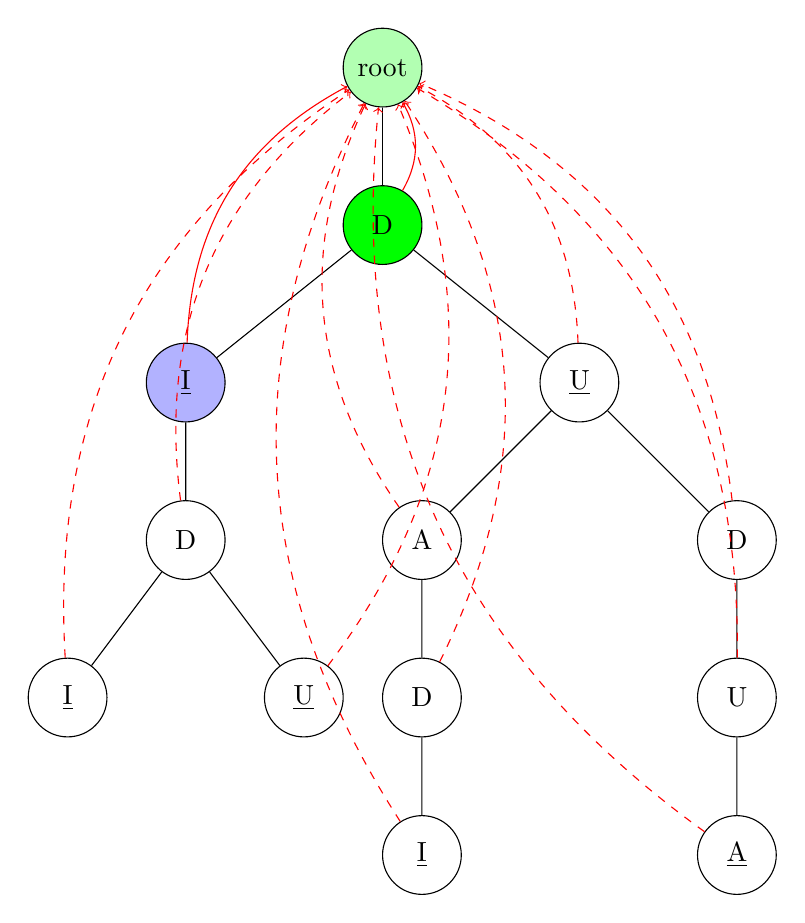
\begin{tikzpicture}[
        level 1/.style={sibling distance=6cm, level distance=2cm},
        level 2/.style={sibling distance=5cm, level distance=2cm},
        level 3/.style={sibling distance=4cm, level distance=2cm},
        level 4/.style={sibling distance=3cm, level distance=2cm},
        level 5/.style={sibling distance=2cm, level distance=2cm},
        level 6/.style={sibling distance=2cm, level distance=2ccm},
        every node/.style={circle, draw, minimum size=1cm}
    ]
        % Vẽ cây chính
        \node [fill=green!30](root) {root}
            child { node [fill=green](D1) {D}
                child { node [fill=blue!30] (I) {\underline{I}}
                    child { node (D2) {D}
                        child { node (I2) {\underline{I}} }
                        child { node (U2) {\underline{U}} }
                    }
                }
                child { node (U1) {\underline{U}}
                    child { node (A2) {A}
                        child { node (D4) {D}
                            child { node (I3) {\underline{I}} }
                        }
                    }
                    child { node (D3) {D}
                        child { node (U3) {U}
                            child { node (A) {\underline{A}} }
                        }
                    }
                }
            };

        % Thêm các liên kết về gốc
        \draw[red, ->] (D1) to[bend right] (root);
        \draw[red, ->] (I) to[bend left] (root);
        \draw[red, dashed, ->] (I2) to[bend left] (root);
        \draw[red, dashed, ->] (D2) to[bend left] (root);
        \draw[red, dashed, ->] (U1) to[bend right] (root);
        \draw[red, dashed, ->] (D3) to[bend right] (root);
        \draw[red, dashed, ->] (U2) to[bend right] (root);
        \draw[red, dashed, ->] (A) to[bend left] (root);
        \draw[red, dashed, ->] (A2) to[bend left] (root);
        \draw[red, dashed, ->] (D4) to[bend right] (root);
        \draw[red, dashed, ->] (I3) to[bend left] (root);
        \draw[red, dashed, ->] (U3) to[bend right] (root);
    \end{tikzpicture}

    Travel to node I. The parent of this node is node D. 
    
    The suffix link of node D points to the root. 
    
    The root doesn't have node I as its child so we do nothing
\end{center}
\pagebreak

\textbf{Step 3:}
\begin{center}
    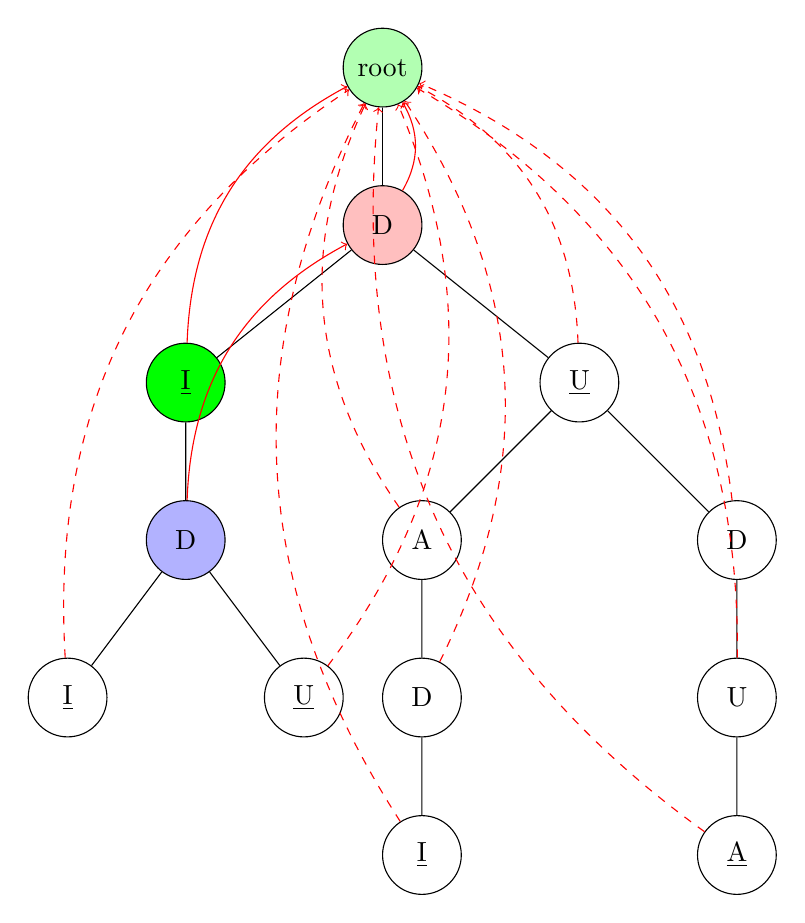
\begin{tikzpicture}[
        level 1/.style={sibling distance=6cm, level distance=2cm},
        level 2/.style={sibling distance=5cm, level distance=2cm},
        level 3/.style={sibling distance=4cm, level distance=2cm},
        level 4/.style={sibling distance=3cm, level distance=2cm},
        level 5/.style={sibling distance=2cm, level distance=2cm},
        level 6/.style={sibling distance=2cm, level distance=2ccm},
        every node/.style={circle, draw, minimum size=1cm}
    ]
        % Vẽ cây chính
        \node [fill=green!30](root) {root}
            child { node [fill=pink](D1) {D}
                child { node [fill=green] (I) {\underline{I}}
                    child { node [fill=blue!30](D2) {D}
                        child { node (I2) {\underline{I}} }
                        child { node (U2) {\underline{U}} }
                    }
                }
                child { node (U1) {\underline{U}}
                    child { node (A2) {A}
                        child { node (D4) {D}
                            child { node (I3) {\underline{I}} }
                        }
                    }
                    child { node (D3) {D}
                        child { node (U3) {U}
                            child { node (A) {\underline{A}} }
                        }
                    }
                }
            };

        % Thêm các liên kết về gốc
        \draw[red, ->] (D1) to[bend right] (root);
        \draw[red, ->] (I) to[bend left] (root);
        \draw[red, dashed, ->] (I2) to[bend left] (root);
        \draw[red, ->] (D2) to[bend left] (D1);
        \draw[red, dashed, ->] (U1) to[bend right] (root);
        \draw[red, dashed, ->] (D3) to[bend right] (root);
        \draw[red, dashed, ->] (U2) to[bend right] (root);
        \draw[red, dashed, ->] (A) to[bend left] (root);
        \draw[red, dashed, ->] (A2) to[bend left] (root);
        \draw[red, dashed, ->] (D4) to[bend right] (root);
        \draw[red, dashed, ->] (I3) to[bend left] (root);
        \draw[red, dashed, ->] (U3) to[bend right] (root);
    \end{tikzpicture}

\end{center}
Travel to node D. The parent of this node is node I. 
    
The suffix link of node I points to the root. 
    
The root has node D as its child so the suffix link is now pointing to that node.
\pagebreak

\textbf{Step 4:}
\begin{center}
    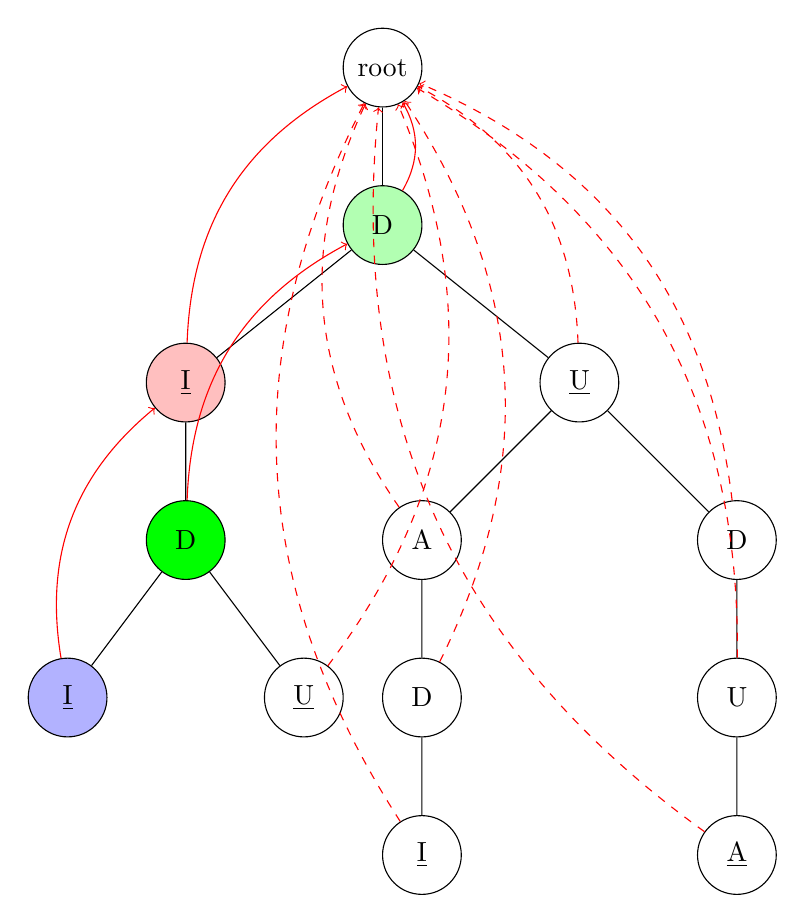
\begin{tikzpicture}[
        level 1/.style={sibling distance=6cm, level distance=2cm},
        level 2/.style={sibling distance=5cm, level distance=2cm},
        level 3/.style={sibling distance=4cm, level distance=2cm},
        level 4/.style={sibling distance=3cm, level distance=2cm},
        level 5/.style={sibling distance=2cm, level distance=2cm},
        level 6/.style={sibling distance=2cm, level distance=2ccm},
        every node/.style={circle, draw, minimum size=1cm}
    ]
        % Vẽ cây chính
        \node (root) {root}
            child { node [fill=green!30](D1) {D}
                child { node [fill=pink](I) {\underline{I}}
                    child { node [fill=green](D2) {D}
                        child { node [fill=blue!30](I2) {\underline{I}} }
                        child { node (U2) {\underline{U}} }
                    }
                }
                child { node (U1) {\underline{U}}
                    child { node (A2) {A}
                        child { node (D4) {D}
                            child { node (I3) {\underline{I}} }
                        }
                    }
                    child { node (D3) {D}
                        child { node (U3) {U}
                            child { node (A) {\underline{A}} }
                        }
                    }
                }
            };

        % Thêm các liên kết về gốc
        \draw[red, ->] (D1) to[bend right] (root);
        \draw[red, ->] (I) to[bend left] (root);
        \draw[red, ->] (I2) to[bend left] (I);
        \draw[red, ->] (D2) to[bend left] (D1);
        \draw[red, dashed, ->] (U1) to[bend right] (root);
        \draw[red, dashed, ->] (D3) to[bend right] (root);
        \draw[red, dashed, ->] (U2) to[bend right] (root);
        \draw[red, dashed, ->] (A) to[bend left] (root);
        \draw[red, dashed, ->] (A2) to[bend left] (root);
        \draw[red, dashed, ->] (D4) to[bend right] (root);
        \draw[red, dashed, ->] (I3) to[bend left] (root);
        \draw[red, dashed, ->] (U3) to[bend right] (root);
    \end{tikzpicture}

\end{center}
Travel to node I. The parent of this node is node D. 
    
The suffix link of node D points to the other node D. 
    
The other node D has node U as its child so the suffix link is now pointing to that node.
\pagebreak

\textbf{Step 5:}
\begin{center}
    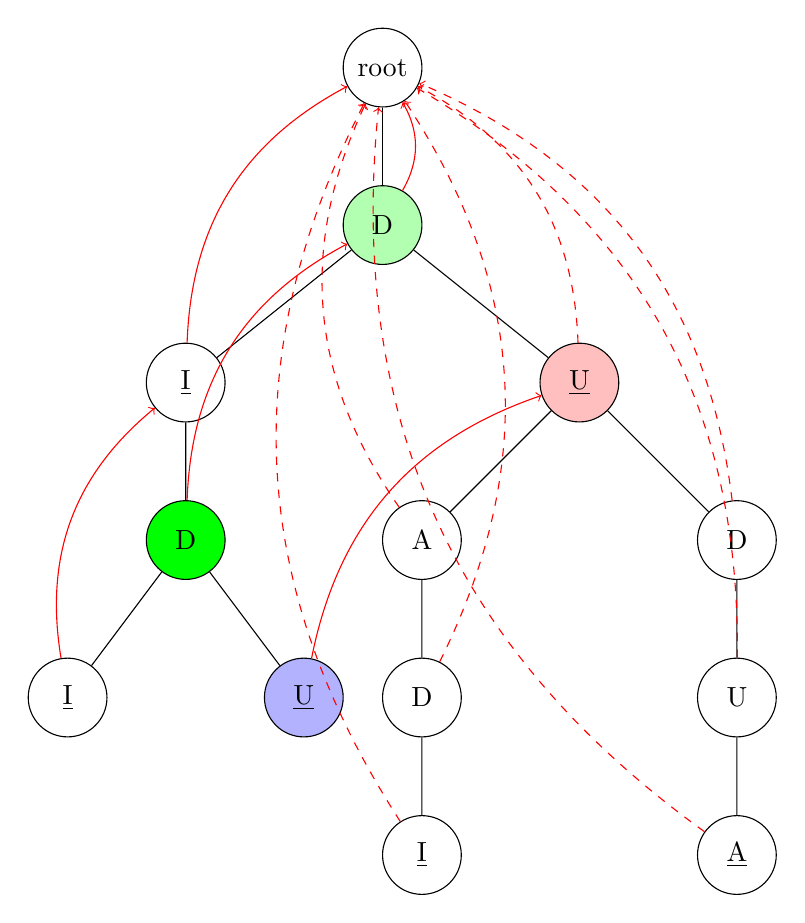
\begin{tikzpicture}[
        level 1/.style={sibling distance=6cm, level distance=2cm},
        level 2/.style={sibling distance=5cm, level distance=2cm},
        level 3/.style={sibling distance=4cm, level distance=2cm},
        level 4/.style={sibling distance=3cm, level distance=2cm},
        level 5/.style={sibling distance=2cm, level distance=2cm},
        level 6/.style={sibling distance=2cm, level distance=2ccm},
        every node/.style={circle, draw, minimum size=1cm}
    ]
        % Vẽ cây chính
        \node (root) {root}
            child { node [fill=green!30](D1) {D}
                child { node (I) {\underline{I}}
                    child { node [fill=green](D2) {D}
                        child { node (I2) {\underline{I}} }
                        child { node [fill=blue!30](U2) {\underline{U}} }
                    }
                }
                child { node [fill=pink](U1) {\underline{U}}
                    child { node (A2) {A}
                        child { node (D4) {D}
                            child { node (I3) {\underline{I}} }
                        }
                    }
                    child { node (D3) {D}
                        child { node (U3) {U}
                            child { node (A) {\underline{A}} }
                        }
                    }
                }
            };

        % Thêm các liên kết về gốc
        \draw[red, ->] (D1) to[bend right] (root);
        \draw[red, ->] (I) to[bend left] (root);
        \draw[red, ->] (I2) to[bend left] (I);
        \draw[red, ->] (D2) to[bend left] (D1);
        \draw[red, dashed, ->] (U1) to[bend right] (root);
        \draw[red, dashed, ->] (D3) to[bend right] (root);
        \draw[red, ->] (U2) to[bend left] (U1);
        \draw[red, dashed, ->] (A) to[bend left] (root);
        \draw[red, dashed, ->] (A2) to[bend left] (root);
        \draw[red, dashed, ->] (D4) to[bend right] (root);
        \draw[red, dashed, ->] (I3) to[bend left] (root);
        \draw[red, dashed, ->] (U3) to[bend right] (root);
    \end{tikzpicture}

\end{center}
Travel to node U. The parent of this node is node D. 
    
The suffix link of node D points to the other node D. 

The other node D has node U as its child so the suffix link is now pointing to that node.
\pagebreak

\textbf{Step 6:}
\begin{center}
    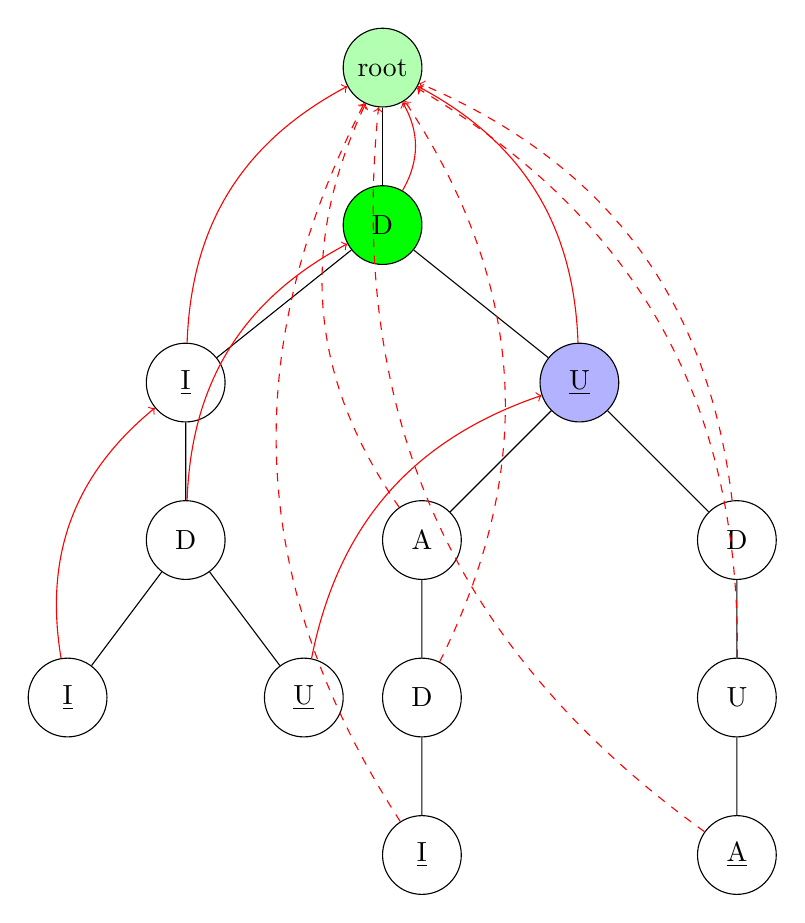
\begin{tikzpicture}[
        level 1/.style={sibling distance=6cm, level distance=2cm},
        level 2/.style={sibling distance=5cm, level distance=2cm},
        level 3/.style={sibling distance=4cm, level distance=2cm},
        level 4/.style={sibling distance=3cm, level distance=2cm},
        level 5/.style={sibling distance=2cm, level distance=2cm},
        level 6/.style={sibling distance=2cm, level distance=2ccm},
        every node/.style={circle, draw, minimum size=1cm}
    ]
        % Vẽ cây chính
        \node [fill=green!30](root) {root}
            child { node [fill=green](D1) {D}
                child { node (I) {\underline{I}}
                    child { node (D2) {D}
                        child { node (I2) {\underline{I}} }
                        child { node (U2) {\underline{U}} }
                    }
                }
                child { node [fill=blue!30](U1) {\underline{U}}
                    child { node (A2) {A}
                        child { node (D4) {D}
                            child { node (I3) {\underline{I}} }
                        }
                    }
                    child { node (D3) {D}
                        child { node (U3) {U}
                            child { node (A) {\underline{A}} }
                        }
                    }
                }
            };

        % Thêm các liên kết về gốc
        \draw[red, ->] (D1) to[bend right] (root);
        \draw[red, ->] (I) to[bend left] (root);
        \draw[red, ->] (I2) to[bend left] (I);
        \draw[red, ->] (D2) to[bend left] (D1);
        \draw[red, ->] (U1) to[bend right] (root);
        \draw[red, dashed, ->] (D3) to[bend right] (root);
        \draw[red, ->] (U2) to[bend left] (U1);
        \draw[red, dashed, ->] (A) to[bend left] (root);
        \draw[red, dashed, ->] (A2) to[bend left] (root);
        \draw[red, dashed, ->] (D4) to[bend right] (root);
        \draw[red, dashed, ->] (I3) to[bend left] (root);
        \draw[red, dashed, ->] (U3) to[bend right] (root);
    \end{tikzpicture}

\end{center}
Travel to node U. The parent of this node is node D. 
    
The suffix link of node D points to the root. 
    
The root doesn't have node U as its child node so we do nothing.
\pagebreak

\textbf{Step 7:}
\begin{center}
    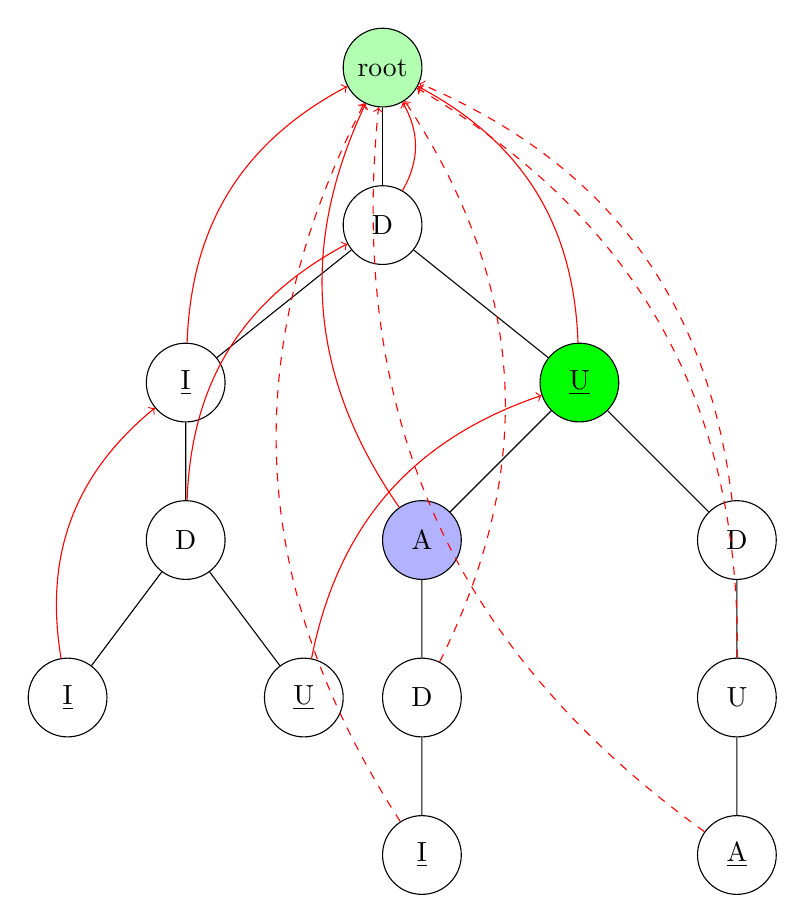
\begin{tikzpicture}[
        level 1/.style={sibling distance=6cm, level distance=2cm},
        level 2/.style={sibling distance=5cm, level distance=2cm},
        level 3/.style={sibling distance=4cm, level distance=2cm},
        level 4/.style={sibling distance=3cm, level distance=2cm},
        level 5/.style={sibling distance=2cm, level distance=2cm},
        level 6/.style={sibling distance=2cm, level distance=2ccm},
        every node/.style={circle, draw, minimum size=1cm}
    ]
        % Vẽ cây chính
        \node [fill=green!30](root) {root}
            child { node (D1) {D}
                child { node (I) {\underline{I}}
                    child { node (D2) {D}
                        child { node (I2) {\underline{I}} }
                        child { node (U2) {\underline{U}} }
                    }
                }
                child { node [fill=green](U1) {\underline{U}}
                    child { node [fill=blue!30](A2) {A}
                        child { node (D4) {D}
                            child { node (I3) {\underline{I}} }
                        }
                    }
                    child { node (D3) {D}
                        child { node (U3) {U}
                            child { node (A) {\underline{A}} }
                        }
                    }
                }
            };

        % Thêm các liên kết về gốc
        \draw[red, ->] (D1) to[bend right] (root);
        \draw[red, ->] (I) to[bend left] (root);
        \draw[red, ->] (I2) to[bend left] (I);
        \draw[red, ->] (D2) to[bend left] (D1);
        \draw[red, ->] (U1) to[bend right] (root);
        \draw[red, dashed, ->] (D3) to[bend right] (root);
        \draw[red, ->] (U2) to[bend left] (U1);
        \draw[red, dashed, ->] (A) to[bend left] (root);
        \draw[red, ->] (A2) to[bend left] (root);
        \draw[red, dashed, ->] (D4) to[bend right] (root);
        \draw[red, dashed, ->] (I3) to[bend left] (root);
        \draw[red, dashed, ->] (U3) to[bend right] (root);
    \end{tikzpicture}

\end{center}
Travel to node A. The parent of this node is node U. 
    
The suffix link of node U points to the root. 
    
The root doesn't have node A as its child node so we do nothing.
\pagebreak

\textbf{Step 8:}
\begin{center}
    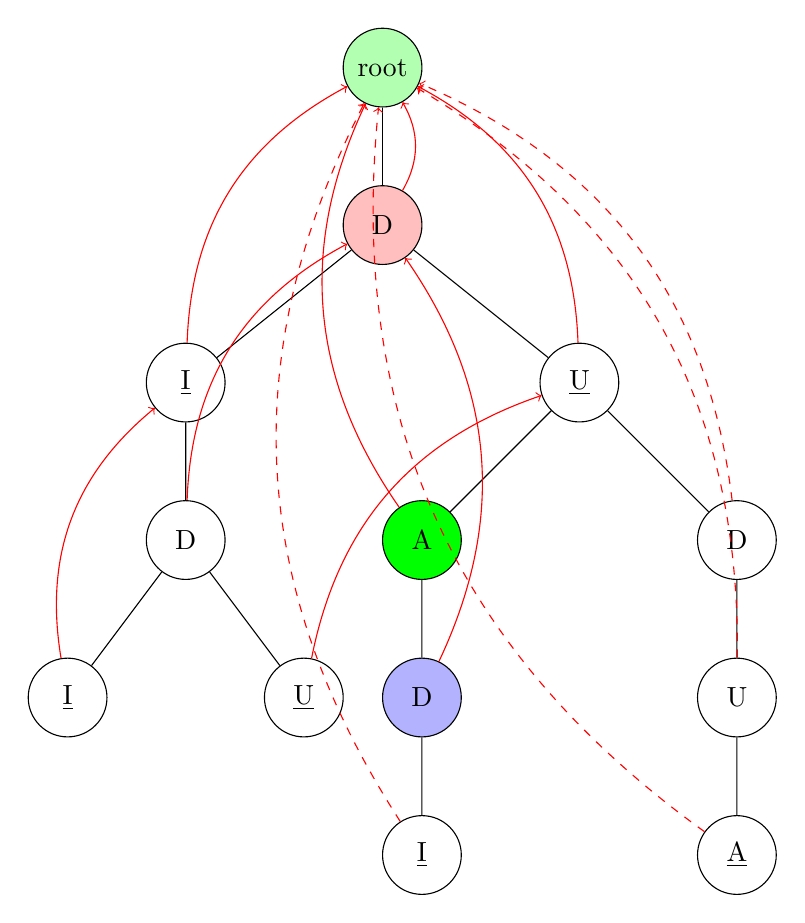
\begin{tikzpicture}[
        level 1/.style={sibling distance=6cm, level distance=2cm},
        level 2/.style={sibling distance=5cm, level distance=2cm},
        level 3/.style={sibling distance=4cm, level distance=2cm},
        level 4/.style={sibling distance=3cm, level distance=2cm},
        level 5/.style={sibling distance=2cm, level distance=2cm},
        level 6/.style={sibling distance=2cm, level distance=2ccm},
        every node/.style={circle, draw, minimum size=1cm}
    ]
        % Vẽ cây chính
        \node [fill=green!30](root) {root}
            child { node [fill=pink](D1) {D}
                child { node (I) {\underline{I}}
                    child { node (D2) {D}
                        child { node (I2) {\underline{I}} }
                        child { node (U2) {\underline{U}} }
                    }
                }
                child { node (U1) {\underline{U}}
                    child { node [fill=green](A2) {A}
                        child { node [fill=blue!30](D4) {D}
                            child { node (I3) {\underline{I}} }
                        }
                    }
                    child { node (D3) {D}
                        child { node (U3) {U}
                            child { node (A) {\underline{A}} }
                        }
                    }
                }
            };

        % Thêm các liên kết về gốc
        \draw[red, ->] (D1) to[bend right] (root);
        \draw[red, ->] (I) to[bend left] (root);
        \draw[red, ->] (I2) to[bend left] (I);
        \draw[red, ->] (D2) to[bend left] (D1);
        \draw[red, ->] (U1) to[bend right] (root);
        \draw[red, dashed, ->] (D3) to[bend right] (root);
        \draw[red, ->] (U2) to[bend left] (U1);
        \draw[red, dashed, ->] (A) to[bend left] (root);
        \draw[red, ->] (A2) to[bend left] (root);
        \draw[red, ->] (D4) to[bend right] (D1);
        \draw[red, dashed, ->] (I3) to[bend left] (root);
        \draw[red, dashed, ->] (U3) to[bend right] (root);
    \end{tikzpicture}

\end{center}
Travel to node D. The parent of this node is node A. 
    
The suffix link of node A points to the root. 
    
The root has node D as its child node so the suffix link is now pointing to that node.
\pagebreak

\textbf{Step 9:}
\begin{center}
    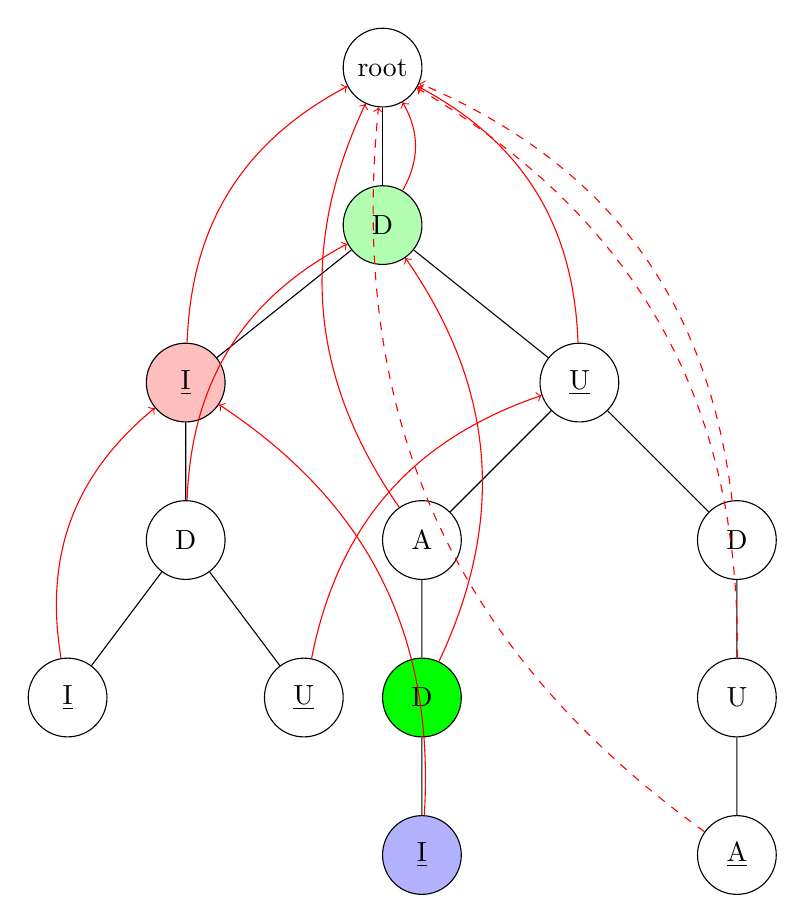
\begin{tikzpicture}[
        level 1/.style={sibling distance=6cm, level distance=2cm},
        level 2/.style={sibling distance=5cm, level distance=2cm},
        level 3/.style={sibling distance=4cm, level distance=2cm},
        level 4/.style={sibling distance=3cm, level distance=2cm},
        level 5/.style={sibling distance=2cm, level distance=2cm},
        level 6/.style={sibling distance=2cm, level distance=2ccm},
        every node/.style={circle, draw, minimum size=1cm}
    ]
        % Vẽ cây chính
        \node (root) {root}
            child { node [fill=green!30](D1) {D}
                child { node [fill=pink](I) {\underline{I}}
                    child { node (D2) {D}
                        child { node (I2) {\underline{I}} }
                        child { node (U2) {\underline{U}} }
                    }
                }
                child { node (U1) {\underline{U}}
                    child { node (A2) {A}
                        child { node [fill=green](D4) {D}
                            child { node [fill=blue!30](I3) {\underline{I}} }
                        }
                    }
                    child { node (D3) {D}
                        child { node (U3) {U}
                            child { node (A) {\underline{A}} }
                        }
                    }
                }
            };

        % Thêm các liên kết về gốc
        \draw[red, ->] (D1) to[bend right] (root);
        \draw[red, ->] (I) to[bend left] (root);
        \draw[red, ->] (I2) to[bend left] (I);
        \draw[red, ->] (D2) to[bend left] (D1);
        \draw[red, ->] (U1) to[bend right] (root);
        \draw[red, dashed, ->] (D3) to[bend right] (root);
        \draw[red, ->] (U2) to[bend left] (U1);
        \draw[red, dashed, ->] (A) to[bend left] (root);
        \draw[red, ->] (A2) to[bend left] (root);
        \draw[red, ->] (D4) to[bend right] (D1);
        \draw[red, ->] (I3) to[bend right] (I);
        \draw[red, dashed, ->] (U3) to[bend right] (root);
    \end{tikzpicture}

\end{center}
Travel to node I. The parent of this node is node I. 
    
The suffix link of node D points to the other node D. 
    
The other node D has node I as its child node so the suffix link is now pointing to that node.
\pagebreak

\textbf{Step 10:}
\begin{center}
    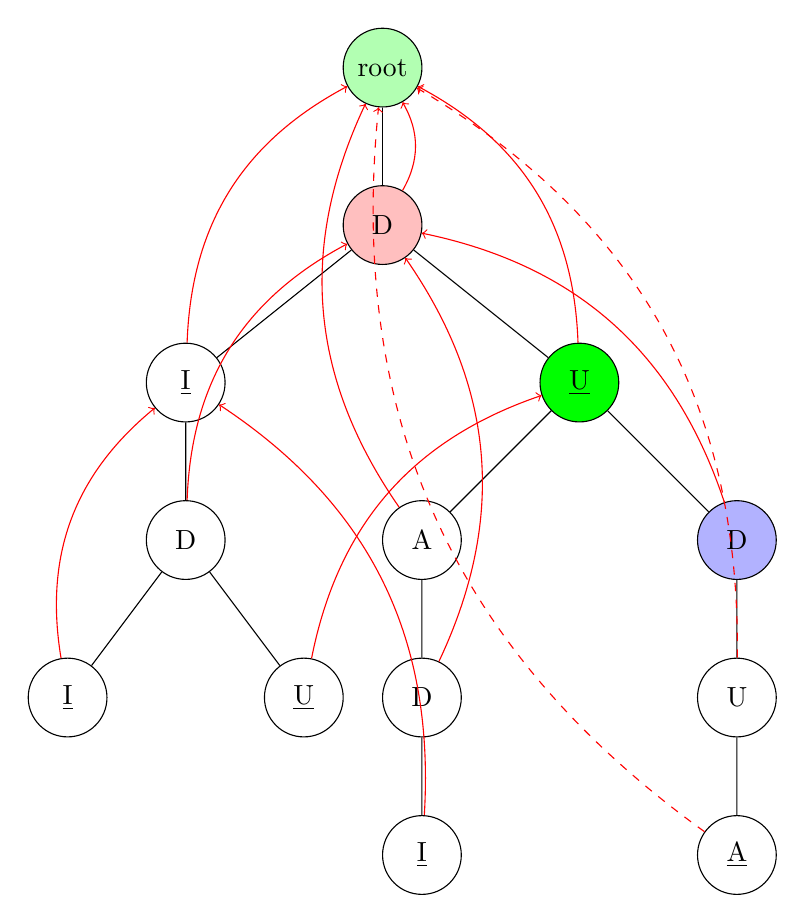
\begin{tikzpicture}[
        level 1/.style={sibling distance=6cm, level distance=2cm},
        level 2/.style={sibling distance=5cm, level distance=2cm},
        level 3/.style={sibling distance=4cm, level distance=2cm},
        level 4/.style={sibling distance=3cm, level distance=2cm},
        level 5/.style={sibling distance=2cm, level distance=2cm},
        level 6/.style={sibling distance=2cm, level distance=2ccm},
        every node/.style={circle, draw, minimum size=1cm}
    ]
        % Vẽ cây chính
        \node [fill=green!30](root) {root}
            child { node [fill=pink](D1) {D}
                child { node (I) {\underline{I}}
                    child { node (D2) {D}
                        child { node (I2) {\underline{I}} }
                        child { node (U2) {\underline{U}} }
                    }
                }
                child { node [fill=green](U1) {\underline{U}}
                    child { node (A2) {A}
                        child { node (D4) {D}
                            child { node (I3) {\underline{I}} }
                        }
                    }
                    child { node [fill=blue!30](D3) {D}
                        child { node (U3) {U}
                            child { node (A) {\underline{A}} }
                        }
                    }
                }
            };

        % Thêm các liên kết về gốc
        \draw[red, ->] (D1) to[bend right] (root);
        \draw[red, ->] (I) to[bend left] (root);
        \draw[red, ->] (I2) to[bend left] (I);
        \draw[red, ->] (D2) to[bend left] (D1);
        \draw[red, ->] (U1) to[bend right] (root);
        \draw[red, ->] (D3) to[bend right] (D1);
        \draw[red, ->] (U2) to[bend left] (U1);
        \draw[red, dashed, ->] (A) to[bend left] (root);
        \draw[red, ->] (A2) to[bend left] (root);
        \draw[red, ->] (D4) to[bend right] (D1);
        \draw[red, ->] (I3) to[bend right] (I);
        \draw[red, dashed, ->] (U3) to[bend right] (root);
    \end{tikzpicture}

\end{center}
Travel to node D. The parent of this node is node U. 
    
The suffix link of node U points to the root. 
    
The root has node D as its child node so the suffix link is now pointing to that node.
\pagebreak

\textbf{Step 11:}
\begin{center}
    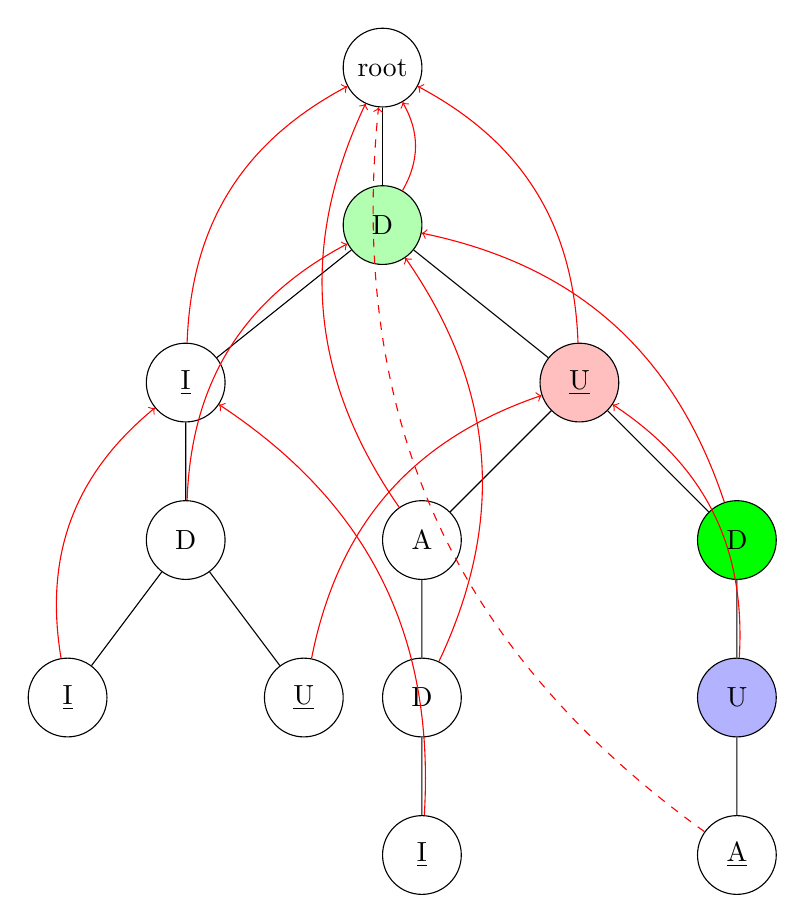
\begin{tikzpicture}[
        level 1/.style={sibling distance=6cm, level distance=2cm},
        level 2/.style={sibling distance=5cm, level distance=2cm},
        level 3/.style={sibling distance=4cm, level distance=2cm},
        level 4/.style={sibling distance=3cm, level distance=2cm},
        level 5/.style={sibling distance=2cm, level distance=2cm},
        level 6/.style={sibling distance=2cm, level distance=2ccm},
        every node/.style={circle, draw, minimum size=1cm}
    ]
        % Vẽ cây chính
        \node (root) {root}
            child { node [fill=green!30](D1) {D}
                child { node (I) {\underline{I}}
                    child { node (D2) {D}
                        child { node (I2) {\underline{I}} }
                        child { node (U2) {\underline{U}} }
                    }
                }
                child { node [fill=pink](U1) {\underline{U}}
                    child { node (A2) {A}
                        child { node (D4) {D}
                            child { node (I3) {\underline{I}} }
                        }
                    }
                    child { node [fill=green](D3) {D}
                        child { node[fill=blue!30] (U3) {U}
                            child { node (A) {\underline{A}} }
                        }
                    }
                }
            };

        % Thêm các liên kết về gốc
        \draw[red, ->] (D1) to[bend right] (root);
        \draw[red, ->] (I) to[bend left] (root);
        \draw[red, ->] (I2) to[bend left] (I);
        \draw[red, ->] (D2) to[bend left] (D1);
        \draw[red, ->] (U1) to[bend right] (root);
        \draw[red, ->] (D3) to[bend right] (D1);
        \draw[red, ->] (U2) to[bend left] (U1);
        \draw[red, dashed, ->] (A) to[bend left] (root);
        \draw[red, ->] (A2) to[bend left] (root);
        \draw[red, ->] (D4) to[bend right] (D1);
        \draw[red, ->] (I3) to[bend right] (I);
        \draw[red, ->] (U3) to[bend right] (U1);
    \end{tikzpicture}

\end{center}
Travel to node U. The parent of this node is node D. 
    
The suffix link of node D points to the other node D. 
    
The other node D has node U as its child node so the suffix link is now pointing to that node.
\pagebreak

\textbf{Step 12:}
\begin{center}
    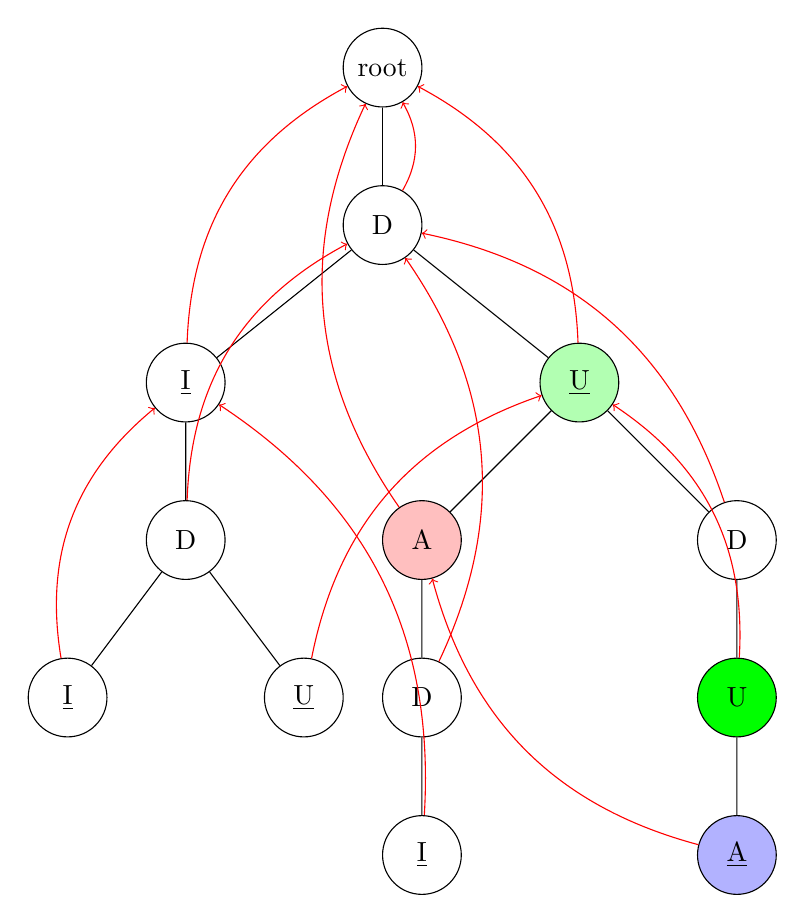
\begin{tikzpicture}[
        level 1/.style={sibling distance=6cm, level distance=2cm},
        level 2/.style={sibling distance=5cm, level distance=2cm},
        level 3/.style={sibling distance=4cm, level distance=2cm},
        level 4/.style={sibling distance=3cm, level distance=2cm},
        level 5/.style={sibling distance=2cm, level distance=2cm},
        level 6/.style={sibling distance=2cm, level distance=2ccm},
        every node/.style={circle, draw, minimum size=1cm}
    ]
        % Vẽ cây chính
        \node (root) {root}
            child { node (D1) {D}
                child { node (I) {\underline{I}}
                    child { node (D2) {D}
                        child { node (I2) {\underline{I}} }
                        child { node (U2) {\underline{U}} }
                    }
                }
                child { node [fill=green!30](U1) {\underline{U}}
                    child { node [fill=pink](A2) {A}
                        child { node (D4) {D}
                            child { node (I3) {\underline{I}} }
                        }
                    }
                    child { node (D3) {D}
                        child { node[fill=green] (U3) {U}
                            child { node [fill=blue!30](A) {\underline{A}} }
                        }
                    }
                }
            };

        % Thêm các liên kết về gốc
        \draw[red, ->] (D1) to[bend right] (root);
        \draw[red, ->] (I) to[bend left] (root);
        \draw[red, ->] (I2) to[bend left] (I);
        \draw[red, ->] (D2) to[bend left] (D1);
        \draw[red, ->] (U1) to[bend right] (root);
        \draw[red, ->] (D3) to[bend right] (D1);
        \draw[red, ->] (U2) to[bend left] (U1);
        \draw[red, ->] (A) to[bend left] (A2);
        \draw[red, ->] (A2) to[bend left] (root);
        \draw[red, ->] (D4) to[bend right] (D1);
        \draw[red, ->] (I3) to[bend right] (I);
        \draw[red, ->] (U3) to[bend right] (U1);
    \end{tikzpicture}

\end{center}
Travel to node A. The parent of this node is node U. 
    
The suffix link of node U points to the other node U. 
    
The other node U has node A as its child node so the suffix link is now pointing to that node.
\pagebreak
\subsubsection*{Result}
\begin{center}
    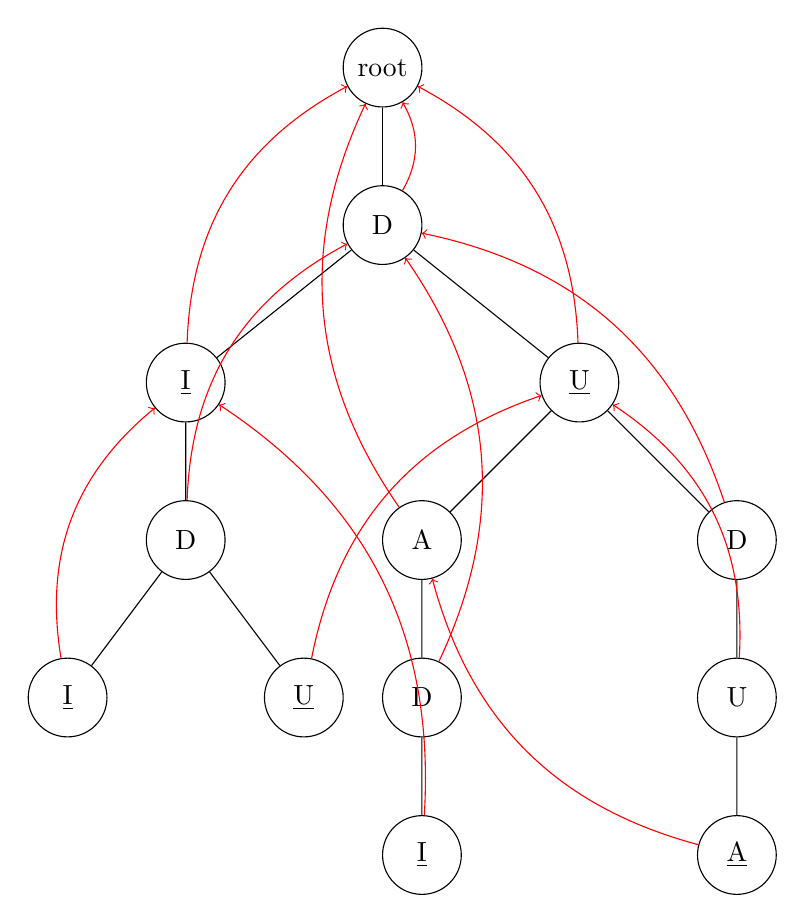
\begin{tikzpicture}[
        level 1/.style={sibling distance=6cm, level distance=2cm},
        level 2/.style={sibling distance=5cm, level distance=2cm},
        level 3/.style={sibling distance=4cm, level distance=2cm},
        level 4/.style={sibling distance=3cm, level distance=2cm},
        level 5/.style={sibling distance=2cm, level distance=2cm},
        level 6/.style={sibling distance=2cm, level distance=2ccm},
        every node/.style={circle, draw, minimum size=1cm}
    ]
        % Vẽ cây chính
        \node (root) {root}
            child { node (D1) {D}
                child { node (I) {\underline{I}}
                    child { node (D2) {D}
                        child { node (I2) {\underline{I}} }
                        child { node (U2) {\underline{U}} }
                    }
                }
                child { node (U1) {\underline{U}}
                    child { node (A2) {A}
                        child { node (D4) {D}
                            child { node (I3) {\underline{I}} }
                        }
                    }
                    child { node (D3) {D}
                        child { node (U3) {U}
                            child { node (A) {\underline{A}} }
                        }
                    }
                }
            };

        % Thêm các liên kết về gốc
        \draw[red, ->] (D1) to[bend right] (root);
        \draw[red, ->] (I) to[bend left] (root);
        \draw[red, ->] (I2) to[bend left] (I);
        \draw[red, ->] (D2) to[bend left] (D1);
        \draw[red, ->] (U1) to[bend right] (root);
        \draw[red, ->] (D3) to[bend right] (D1);
        \draw[red, ->] (U2) to[bend left] (U1);
        \draw[red, ->] (A) to[bend left] (A2);
        \draw[red, ->] (A2) to[bend left] (root);
        \draw[red, ->] (D4) to[bend right] (D1);
        \draw[red, ->] (I3) to[bend right] (I);
        \draw[red, ->] (U3) to[bend right] (U1);
    \end{tikzpicture}
\end{center}
\subsection{Matching/ Searching process}
At this process, we use the character at the position i of the text to travel through trie respectively.

At position i, if the current has the child text[i], we will travel to that child node. Otherwise, we use the suffix link to trace back to the other node to check whether that node has that child text[i]. This procedure repeats until there is a child node text[i] or the node is the root. If the node is the root, the searching process will stop. But there is a child node text[i], we will travel to that node and continue the procedure. 

After travel to that node, if the node is the end of a pattern and we have not counted that pattern, so we count it. Then we trace back using the suffix link procedure until the node is the root to check that all the prefixes are the end of any pattern or not. If there is the end of the pattern and it has not been counted, we count it. 
\pagebreak
\subsubsection*{Source code}
\lstinputlisting[language=C++]{code/traceBack.cpp}
\pagebreak
\subsubsection*{Step by step}
\textbf{Step 1:}
\begin{center}

    \begin{table}[H]
    \centering
    \begin{tabular}{|c|c|c|c|c|c|c|c|c|c|}
    \hline
    pos   & i &   &   &   &   &   &   &   &   \\ \hline
    text  & D & I & D & U & D & U & A & D & I \\ \hline
    \end{tabular}
    \end{table}
    
    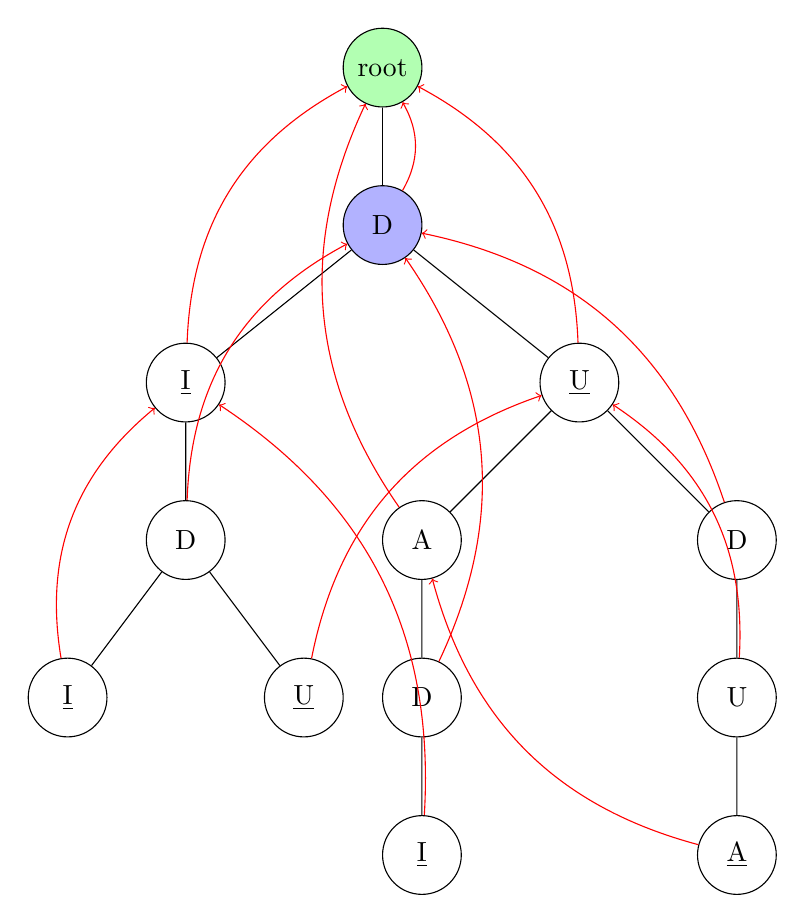
\begin{tikzpicture}[
        level 1/.style={sibling distance=6cm, level distance=2cm},
        level 2/.style={sibling distance=5cm, level distance=2cm},
        level 3/.style={sibling distance=4cm, level distance=2cm},
        level 4/.style={sibling distance=3cm, level distance=2cm},
        level 5/.style={sibling distance=2cm, level distance=2cm},
        level 6/.style={sibling distance=2cm, level distance=2ccm},
        every node/.style={circle, draw, minimum size=1cm}
    ]
        % Vẽ cây chính
        \node [fill=green!30](root) {root}
            child { node [fill=blue!30](D1) {D}
                child { node (I) {\underline{I}}
                    child { node (D2) {D}
                        child { node (I2) {\underline{I}} }
                        child { node (U2) {\underline{U}} }
                    }
                }
                child { node (U1) {\underline{U}}
                    child { node (A2) {A}
                        child { node (D4) {D}
                            child { node (I3) {\underline{I}} }
                        }
                    }
                    child { node (D3) {D}
                        child { node (U3) {U}
                            child { node (A) {\underline{A}} }
                        }
                    }
                }
            };

        % Thêm các liên kết về gốc
        \draw[red, ->] (D1) to[bend right] (root);
        \draw[red, ->] (I) to[bend left] (root);
        \draw[red, ->] (I2) to[bend left] (I);
        \draw[red, ->] (D2) to[bend left] (D1);
        \draw[red, ->] (U1) to[bend right] (root);
        \draw[red, ->] (D3) to[bend right] (D1);
        \draw[red, ->] (U2) to[bend left] (U1);
        \draw[red, ->] (A) to[bend left] (A2);
        \draw[red, ->] (A2) to[bend left] (root);
        \draw[red, ->] (D4) to[bend right] (D1);
        \draw[red, ->] (I3) to[bend right] (I);
        \draw[red, ->] (U3) to[bend right] (U1);
    \end{tikzpicture}

\end{center}
The number of patterns that occur in the text: 0.

Now text[i] = D, we travel to node D from the root. Because node D is not the end of any patterns, we do nothing in this node. We trace back to the node the suffix link of this node points at, which is the root. Because this is the root, we stop the procedure.
\pagebreak

\textbf{Step 2:}
\begin{center}

    \begin{table}[H]
    \centering
    \begin{tabular}{|c|c|c|c|c|c|c|c|c|c|}
    \hline
    pos   &   & i &   &   &   &   &   &   &   \\ \hline
    text  & D & I & D & U & D & U & A & D & I \\ \hline
    \end{tabular}
    \end{table}
    
    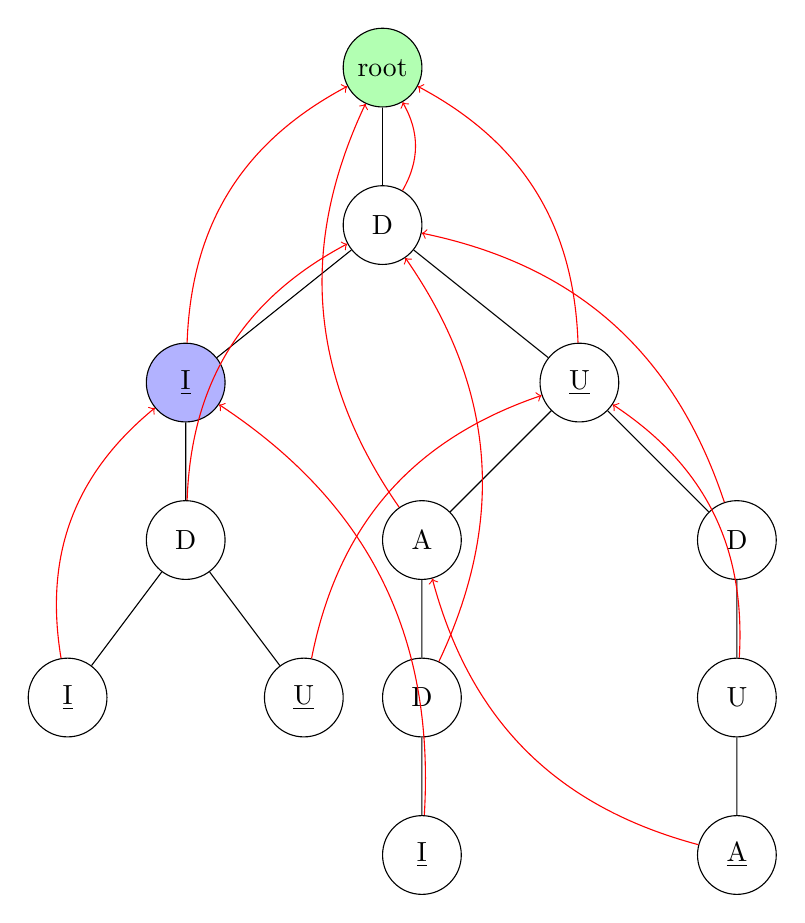
\begin{tikzpicture}[
        level 1/.style={sibling distance=6cm, level distance=2cm},
        level 2/.style={sibling distance=5cm, level distance=2cm},
        level 3/.style={sibling distance=4cm, level distance=2cm},
        level 4/.style={sibling distance=3cm, level distance=2cm},
        level 5/.style={sibling distance=2cm, level distance=2cm},
        level 6/.style={sibling distance=2cm, level distance=2ccm},
        every node/.style={circle, draw, minimum size=1cm}
    ]
        % Vẽ cây chính
        \node [fill=green!30](root) {root}
            child { node (D1) {D}
                child { node [fill=blue!30](I) {\underline{I}}
                    child { node (D2) {D}
                        child { node (I2) {\underline{I}} }
                        child { node (U2) {\underline{U}} }
                    }
                }
                child { node (U1) {\underline{U}}
                    child { node (A2) {A}
                        child { node (D4) {D}
                            child { node (I3) {\underline{I}} }
                        }
                    }
                    child { node (D3) {D}
                        child { node (U3) {U}
                            child { node (A) {\underline{A}} }
                        }
                    }
                }
            };

        % Thêm các liên kết về gốc
        \draw[red, ->] (D1) to[bend right] (root);
        \draw[red, ->] (I) to[bend left] (root);
        \draw[red, ->] (I2) to[bend left] (I);
        \draw[red, ->] (D2) to[bend left] (D1);
        \draw[red, ->] (U1) to[bend right] (root);
        \draw[red, ->] (D3) to[bend right] (D1);
        \draw[red, ->] (U2) to[bend left] (U1);
        \draw[red, ->] (A) to[bend left] (A2);
        \draw[red, ->] (A2) to[bend left] (root);
        \draw[red, ->] (D4) to[bend right] (D1);
        \draw[red, ->] (I3) to[bend right] (I);
        \draw[red, ->] (U3) to[bend right] (U1);
    \end{tikzpicture}

\end{center}
Number of patterns that occur in the text: 1 (DI).

Now text[i] = I, we travel to node I from node D. Because node I is the end of a pattern DI and pattern have not been counted, the number of pattern that occur in the text is increased by 1. We trace back to the node the suffix of this node points at, which is the root, Because this is the root, we stop the procedure.
\pagebreak

\textbf{Step 3:}
\begin{center}

    \begin{table}[H]
    \centering
    \begin{tabular}{|c|c|c|c|c|c|c|c|c|c|}
    \hline
    pos   &   &   & i &   &   &   &   &   &   \\ \hline
    text  & D & I & D & U & D & U & A & D & I \\ \hline
    \end{tabular}
    \end{table}
    
    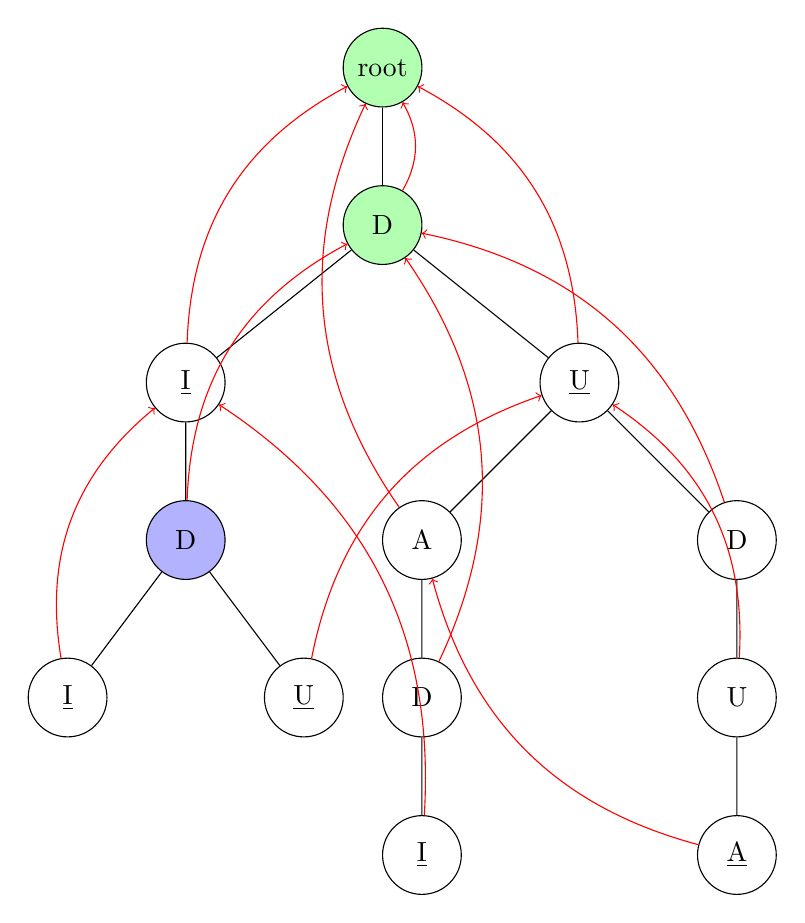
\begin{tikzpicture}[
        level 1/.style={sibling distance=6cm, level distance=2cm},
        level 2/.style={sibling distance=5cm, level distance=2cm},
        level 3/.style={sibling distance=4cm, level distance=2cm},
        level 4/.style={sibling distance=3cm, level distance=2cm},
        level 5/.style={sibling distance=2cm, level distance=2cm},
        level 6/.style={sibling distance=2cm, level distance=2ccm},
        every node/.style={circle, draw, minimum size=1cm}
    ]
        % Vẽ cây chính
        \node [fill=green!30](root) {root}
            child { node [fill=green!30](D1) {D}
                child { node (I) {\underline{I}}
                    child { node [fill=blue!30](D2) {D}
                        child { node (I2) {\underline{I}} }
                        child { node (U2) {\underline{U}} }
                    }
                }
                child { node (U1) {\underline{U}}
                    child { node (A2) {A}
                        child { node (D4) {D}
                            child { node (I3) {\underline{I}} }
                        }
                    }
                    child { node (D3) {D}
                        child { node (U3) {U}
                            child { node (A) {\underline{A}} }
                        }
                    }
                }
            };

        % Thêm các liên kết về gốc
        \draw[red, ->] (D1) to[bend right] (root);
        \draw[red, ->] (I) to[bend left] (root);
        \draw[red, ->] (I2) to[bend left] (I);
        \draw[red, ->] (D2) to[bend left] (D1);
        \draw[red, ->] (U1) to[bend right] (root);
        \draw[red, ->] (D3) to[bend right] (D1);
        \draw[red, ->] (U2) to[bend left] (U1);
        \draw[red, ->] (A) to[bend left] (A2);
        \draw[red, ->] (A2) to[bend left] (root);
        \draw[red, ->] (D4) to[bend right] (D1);
        \draw[red, ->] (I3) to[bend right] (I);
        \draw[red, ->] (U3) to[bend right] (U1);
    \end{tikzpicture}

\end{center}
Number of patterns that occur in the text: 1 (DI).

Now text[i] = D, we travel to node D from node I. Because node D is not the end of nay patterns, we do nothing. We trace back to the node the suffix link of this node points at, which is the other node D. Because node D is not the end of any pattern, we do nothing at this node. We trace back to the node the suffix link of this node points at, which is the root. Because this is the root, we stop the procedure.
\pagebreak

\textbf{Step 4:}
\begin{center}

    \begin{table}[H]
    \centering
    \begin{tabular}{|c|c|c|c|c|c|c|c|c|c|}
    \hline
    pos   &   &   &   & i &   &   &   &   &   \\ \hline
    text  & D & I & D & U & D & U & A & D & I \\ \hline
    \end{tabular}
    \end{table}
    
    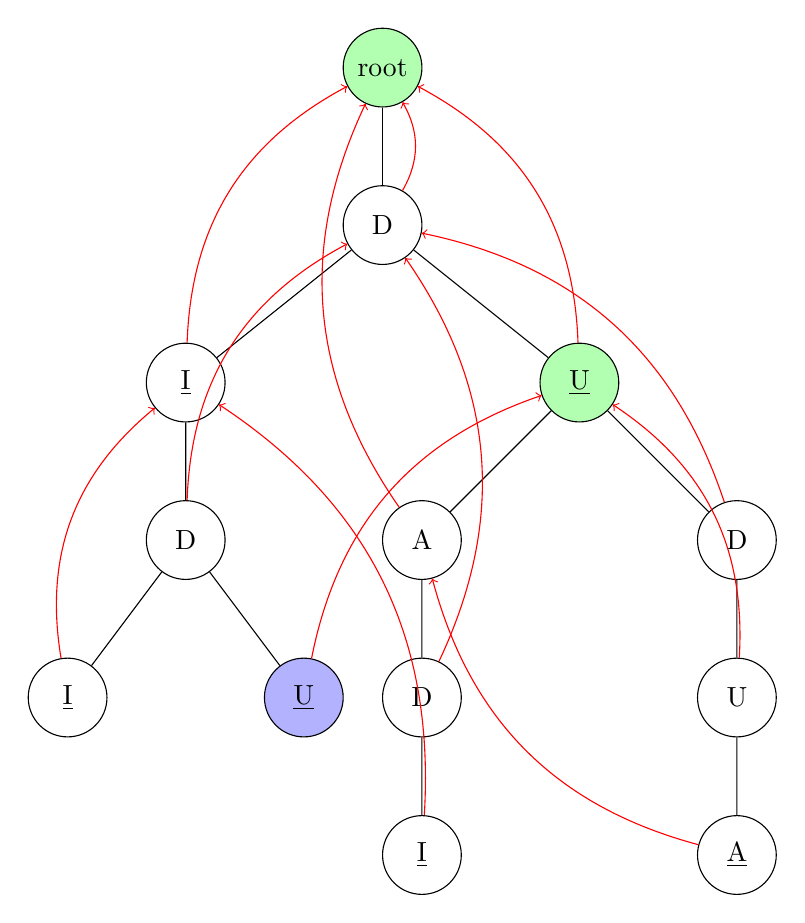
\begin{tikzpicture}[
        level 1/.style={sibling distance=6cm, level distance=2cm},
        level 2/.style={sibling distance=5cm, level distance=2cm},
        level 3/.style={sibling distance=4cm, level distance=2cm},
        level 4/.style={sibling distance=3cm, level distance=2cm},
        level 5/.style={sibling distance=2cm, level distance=2cm},
        level 6/.style={sibling distance=2cm, level distance=2ccm},
        every node/.style={circle, draw, minimum size=1cm}
    ]
        % Vẽ cây chính
        \node [fill=green!30](root) {root}
            child { node (D1) {D}
                child { node (I) {\underline{I}}
                    child { node (D2) {D}
                        child { node (I2) {\underline{I}} }
                        child { node [fill=blue!30](U2) {\underline{U}} }
                    }
                }
                child { node [fill=green!30](U1) {\underline{U}}
                    child { node (A2) {A}
                        child { node (D4) {D}
                            child { node (I3) {\underline{I}} }
                        }
                    }
                    child { node (D3) {D}
                        child { node (U3) {U}
                            child { node (A) {\underline{A}} }
                        }
                    }
                }
            };

        % Thêm các liên kết về gốc
        \draw[red, ->] (D1) to[bend right] (root);
        \draw[red, ->] (I) to[bend left] (root);
        \draw[red, ->] (I2) to[bend left] (I);
        \draw[red, ->] (D2) to[bend left] (D1);
        \draw[red, ->] (U1) to[bend right] (root);
        \draw[red, ->] (D3) to[bend right] (D1);
        \draw[red, ->] (U2) to[bend left] (U1);
        \draw[red, ->] (A) to[bend left] (A2);
        \draw[red, ->] (A2) to[bend left] (root);
        \draw[red, ->] (D4) to[bend right] (D1);
        \draw[red, ->] (I3) to[bend right] (I);
        \draw[red, ->] (U3) to[bend right] (U1);
    \end{tikzpicture}

\end{center}
Number of patterns that occur in the text: 3 (DI, DIDU, DU).

Now text[i] = I, we travel to node U from node D. Because node U is the end of a pattern DIDU and this pattern have not been counted, the number of patterns that occur in the text in increased by 1. We trace back to the node the suffix link of this node points at, which is the other node U. Because node U is the end of pattern DU and this pattern have not been counted, the number of patterns that occur in the text is increased by 1. We trace back to the node the suffix link of this node points at, which is the root. Because this is the root, we stop the procedure.
\pagebreak

\textbf{Step 5:}
\begin{center}

    \begin{table}[H]
    \centering
    \begin{tabular}{|c|c|c|c|c|c|c|c|c|c|}
    \hline
    pos   &   &   &   &   & i &   &   &   &   \\ \hline
    text  & D & I & D & U & D & U & A & D & I \\ \hline
    \end{tabular}
    \end{table}
    
    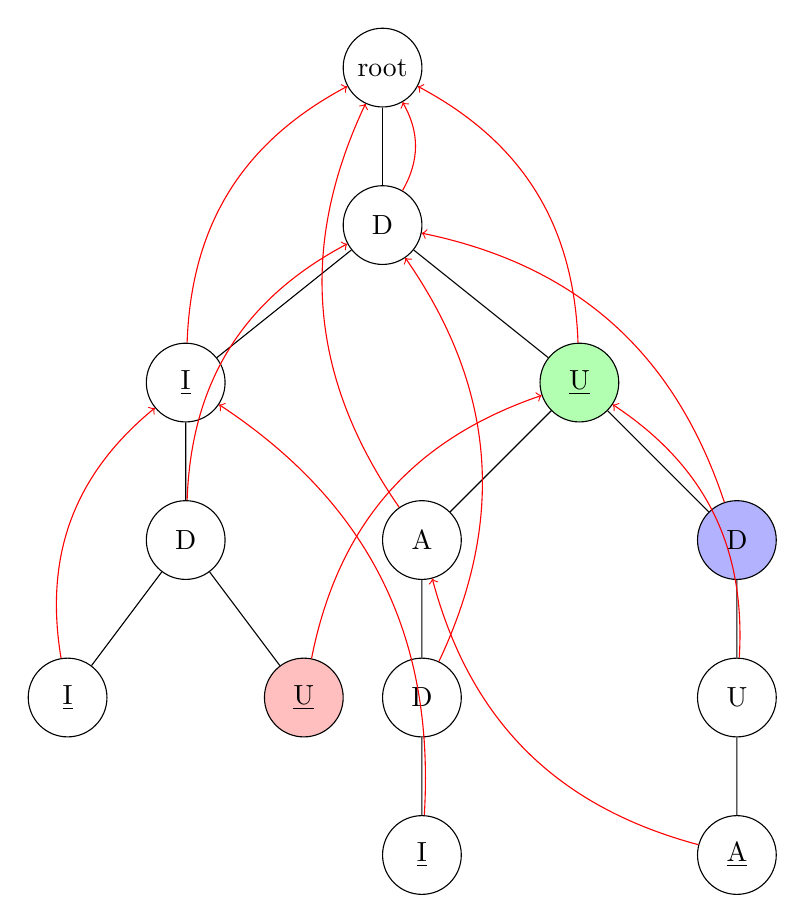
\begin{tikzpicture}[
        level 1/.style={sibling distance=6cm, level distance=2cm},
        level 2/.style={sibling distance=5cm, level distance=2cm},
        level 3/.style={sibling distance=4cm, level distance=2cm},
        level 4/.style={sibling distance=3cm, level distance=2cm},
        level 5/.style={sibling distance=2cm, level distance=2cm},
        level 6/.style={sibling distance=2cm, level distance=2ccm},
        every node/.style={circle, draw, minimum size=1cm}
    ]
        % Vẽ cây chính
        \node (root) {root}
            child { node (D1) {D}
                child { node (I) {\underline{I}}
                    child { node (D2) {D}
                        child { node (I2) {\underline{I}} }
                        child { node [fill=pink](U2) {\underline{U}} }
                    }
                }
                child { node [fill=green!30](U1) {\underline{U}}
                    child { node (A2) {A}
                        child { node (D4) {D}
                            child { node (I3) {\underline{I}} }
                        }
                    }
                    child { node [fill=blue!30](D3) {D}
                        child { node (U3) {U}
                            child { node (A) {\underline{A}} }
                        }
                    }
                }
            };

        % Thêm các liên kết về gốc
        \draw[red, ->] (D1) to[bend right] (root);
        \draw[red, ->] (I) to[bend left] (root);
        \draw[red, ->] (I2) to[bend left] (I);
        \draw[red, ->] (D2) to[bend left] (D1);
        \draw[red, ->] (U1) to[bend right] (root);
        \draw[red, ->] (D3) to[bend right] (D1);
        \draw[red, ->] (U2) to[bend left] (U1);
        \draw[red, ->] (A) to[bend left] (A2);
        \draw[red, ->] (A2) to[bend left] (root);
        \draw[red, ->] (D4) to[bend right] (D1);
        \draw[red, ->] (I3) to[bend right] (I);
        \draw[red, ->] (U3) to[bend right] (U1);
    \end{tikzpicture}

\end{center}
Number of patterns that occur in the text: 3 (DI, DIDU, DU).

Now text[i] = D, but node U doesn't have node child D we trace back to the node the suffix link of node U points at, which points to other node U. That node U has node child D so we travel to that node D.
\pagebreak

\textbf{Step 6:}
\begin{center}

    \begin{table}[H]
    \centering
    \begin{tabular}{|c|c|c|c|c|c|c|c|c|c|}
    \hline
    pos   &   &   &   &   & i &   &   &   &   \\ \hline
    text  & D & I & D & U & D & U & A & D & I \\ \hline
    \end{tabular}
    \end{table}
    
    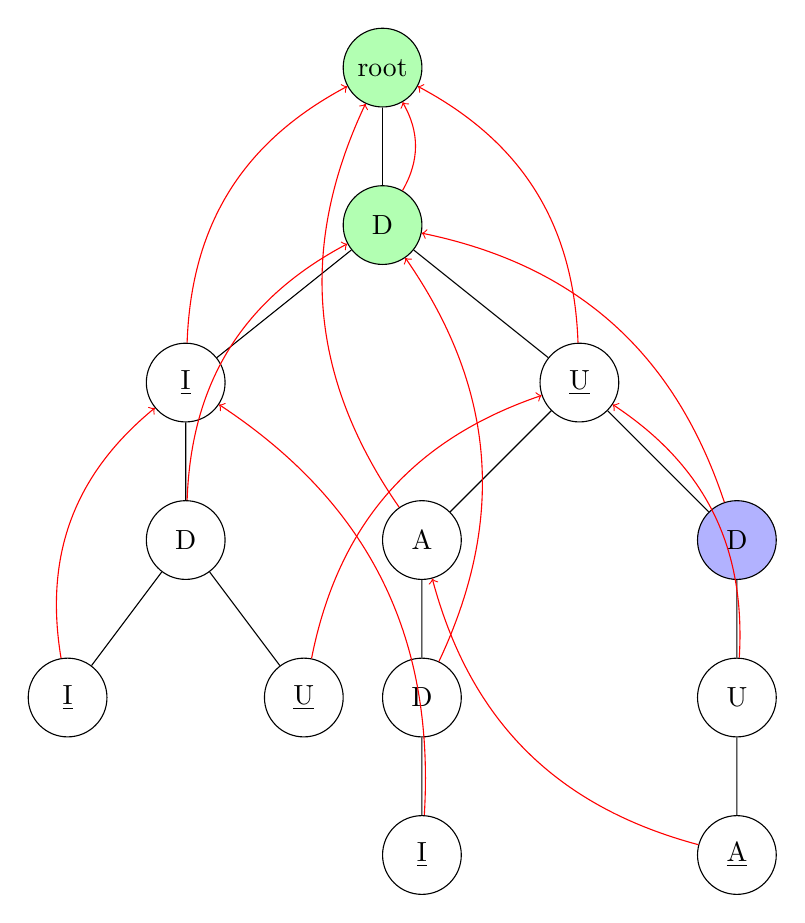
\begin{tikzpicture}[
        level 1/.style={sibling distance=6cm, level distance=2cm},
        level 2/.style={sibling distance=5cm, level distance=2cm},
        level 3/.style={sibling distance=4cm, level distance=2cm},
        level 4/.style={sibling distance=3cm, level distance=2cm},
        level 5/.style={sibling distance=2cm, level distance=2cm},
        level 6/.style={sibling distance=2cm, level distance=2ccm},
        every node/.style={circle, draw, minimum size=1cm}
    ]
        % Vẽ cây chính
        \node [fill=green!30](root) {root}
            child { node [fill=green!30](D1) {D}
                child { node (I) {\underline{I}}
                    child { node (D2) {D}
                        child { node (I2) {\underline{I}} }
                        child { node (U2) {\underline{U}} }
                    }
                }
                child { node (U1) {\underline{U}}
                    child { node (A2) {A}
                        child { node (D4) {D}
                            child { node (I3) {\underline{I}} }
                        }
                    }
                    child { node [fill=blue!30](D3) {D}
                        child { node (U3) {U}
                            child { node (A) {\underline{A}} }
                        }
                    }
                }
            };

        % Thêm các liên kết về gốc
        \draw[red, ->] (D1) to[bend right] (root);
        \draw[red, ->] (I) to[bend left] (root);
        \draw[red, ->] (I2) to[bend left] (I);
        \draw[red, ->] (D2) to[bend left] (D1);
        \draw[red, ->] (U1) to[bend right] (root);
        \draw[red, ->] (D3) to[bend right] (D1);
        \draw[red, ->] (U2) to[bend left] (U1);
        \draw[red, ->] (A) to[bend left] (A2);
        \draw[red, ->] (A2) to[bend left] (root);
        \draw[red, ->] (D4) to[bend right] (D1);
        \draw[red, ->] (I3) to[bend right] (I);
        \draw[red, ->] (U3) to[bend right] (U1);
    \end{tikzpicture}

\end{center}
Number of patterns that occur in the text: 3 (DI, DIDU, DU).

After travel to node D, node D is not the end of any pattern so we do nothing at this node. We trace back to the node the suffix link of this node points at, which is other node D. Because this node is not the end of any pattern, we do nothing on this node. We continue to trace back to the node the suffix link of this node points at, which is the root. Because this is the root, we stop the procedure.
\pagebreak

\textbf{Step 7:}
\begin{center}

    \begin{table}[H]
    \centering
    \begin{tabular}{|c|c|c|c|c|c|c|c|c|c|}
    \hline
    pos   &   &   &   &   &   & i &   &   &   \\ \hline
    text  & D & I & D & U & D & U & A & D & I \\ \hline
    \end{tabular}
    \end{table}
    
    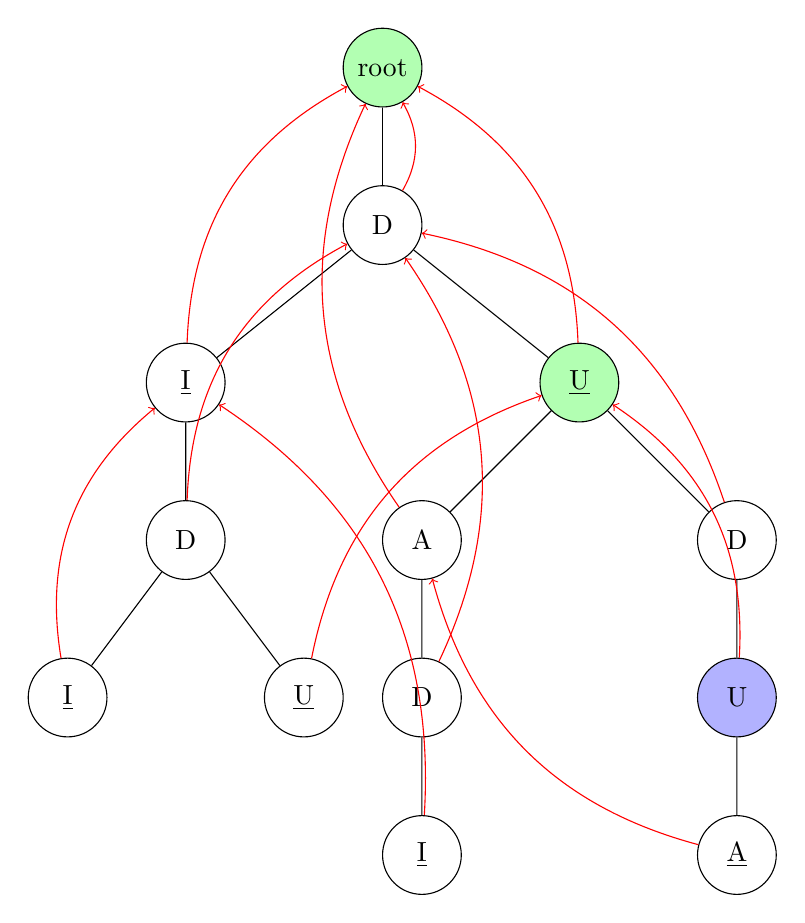
\begin{tikzpicture}[
        level 1/.style={sibling distance=6cm, level distance=2cm},
        level 2/.style={sibling distance=5cm, level distance=2cm},
        level 3/.style={sibling distance=4cm, level distance=2cm},
        level 4/.style={sibling distance=3cm, level distance=2cm},
        level 5/.style={sibling distance=2cm, level distance=2cm},
        level 6/.style={sibling distance=2cm, level distance=2ccm},
        every node/.style={circle, draw, minimum size=1cm}
    ]
        % Vẽ cây chính
        \node [fill=green!30](root) {root}
            child { node (D1) {D}
                child { node (I) {\underline{I}}
                    child { node (D2) {D}
                        child { node (I2) {\underline{I}} }
                        child { node (U2) {\underline{U}} }
                    }
                }
                child { node [fill=green!30](U1) {\underline{U}}
                    child { node (A2) {A}
                        child { node (D4) {D}
                            child { node (I3) {\underline{I}} }
                        }
                    }
                    child { node (D3) {D}
                        child { node [fill=blue!30](U3) {U}
                            child { node (A) {\underline{A}} }
                        }
                    }
                }
            };

        % Thêm các liên kết về gốc
        \draw[red, ->] (D1) to[bend right] (root);
        \draw[red, ->] (I) to[bend left] (root);
        \draw[red, ->] (I2) to[bend left] (I);
        \draw[red, ->] (D2) to[bend left] (D1);
        \draw[red, ->] (U1) to[bend right] (root);
        \draw[red, ->] (D3) to[bend right] (D1);
        \draw[red, ->] (U2) to[bend left] (U1);
        \draw[red, ->] (A) to[bend left] (A2);
        \draw[red, ->] (A2) to[bend left] (root);
        \draw[red, ->] (D4) to[bend right] (D1);
        \draw[red, ->] (I3) to[bend right] (I);
        \draw[red, ->] (U3) to[bend right] (U1);
    \end{tikzpicture}

\end{center}
Number of patterns that occur in the text: 3 (DI, DIDU, DU).

Now text[i] = U, we travel to node U from node D. Because this node is not the end of any pattern, we do nothing on this node. We trace back to the node the suffix link of this node points at, which is other node U. This other node U is the end of pattern DU but this pattern has already counted so we do nothing on this node. We countinue to trace back to the node the suffix of this node points at, which is the root. Because this is the root, we stop the procedure.
\pagebreak

\textbf{Step 8:}
\begin{center}

    \begin{table}[H]
    \centering
    \begin{tabular}{|c|c|c|c|c|c|c|c|c|c|}
    \hline
    pos   &   &   &   &   &   &   & i &   &   \\ \hline
    text  & D & I & D & U & D & U & A & D & I \\ \hline
    \end{tabular}
    \end{table}
    
    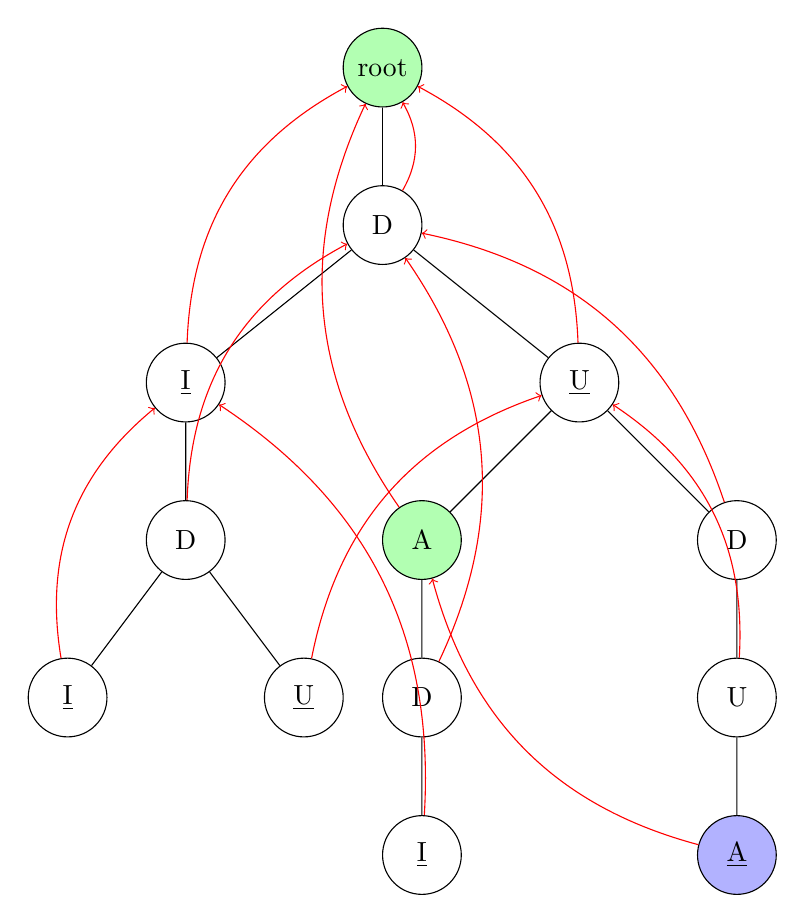
\begin{tikzpicture}[
        level 1/.style={sibling distance=6cm, level distance=2cm},
        level 2/.style={sibling distance=5cm, level distance=2cm},
        level 3/.style={sibling distance=4cm, level distance=2cm},
        level 4/.style={sibling distance=3cm, level distance=2cm},
        level 5/.style={sibling distance=2cm, level distance=2cm},
        level 6/.style={sibling distance=2cm, level distance=2ccm},
        every node/.style={circle, draw, minimum size=1cm}
    ]
        % Vẽ cây chính
        \node [fill=green!30](root) {root}
            child { node (D1) {D}
                child { node (I) {\underline{I}}
                    child { node (D2) {D}
                        child { node (I2) {\underline{I}} }
                        child { node (U2) {\underline{U}} }
                    }
                }
                child { node (U1) {\underline{U}}
                    child { node [fill=green!30](A2) {A}
                        child { node (D4) {D}
                            child { node (I3) {\underline{I}} }
                        }
                    }
                    child { node (D3) {D}
                        child { node (U3) {U}
                            child { node [fill=blue!30](A) {\underline{A}} }
                        }
                    }
                }
            };

        % Thêm các liên kết về gốc
        \draw[red, ->] (D1) to[bend right] (root);
        \draw[red, ->] (I) to[bend left] (root);
        \draw[red, ->] (I2) to[bend left] (I);
        \draw[red, ->] (D2) to[bend left] (D1);
        \draw[red, ->] (U1) to[bend right] (root);
        \draw[red, ->] (D3) to[bend right] (D1);
        \draw[red, ->] (U2) to[bend left] (U1);
        \draw[red, ->] (A) to[bend left] (A2);
        \draw[red, ->] (A2) to[bend left] (root);
        \draw[red, ->] (D4) to[bend right] (D1);
        \draw[red, ->] (I3) to[bend right] (I);
        \draw[red, ->] (U3) to[bend right] (U1);
    \end{tikzpicture}

\end{center}
Number of patterns that occur in the text: 4 (DI, DIDU, DU, DUDUA).

Now text[i] = A, we travel to node A from node U. Because this node is the end of pattern DUDUA and this pattern have not been counted, the number of patterns that occur in the text is increased by 1. We trace back to the node the suffix link of this node points at, which is other node A. This other node A is not the end of any pattern so we do nothing on this node. We countinue to trace back to the node the suffix of this node points at, which is the root. Because this is the root, we stop the procedure.
\pagebreak

\textbf{Step 9:}
\begin{center}

    \begin{table}[H]
    \centering
    \begin{tabular}{|c|c|c|c|c|c|c|c|c|c|}
    \hline
    pos   &   &   &   &   &   & i &   &   &   \\ \hline
    text  & D & I & D & U & D & U & A & D & I \\ \hline
    \end{tabular}
    \end{table}
    
    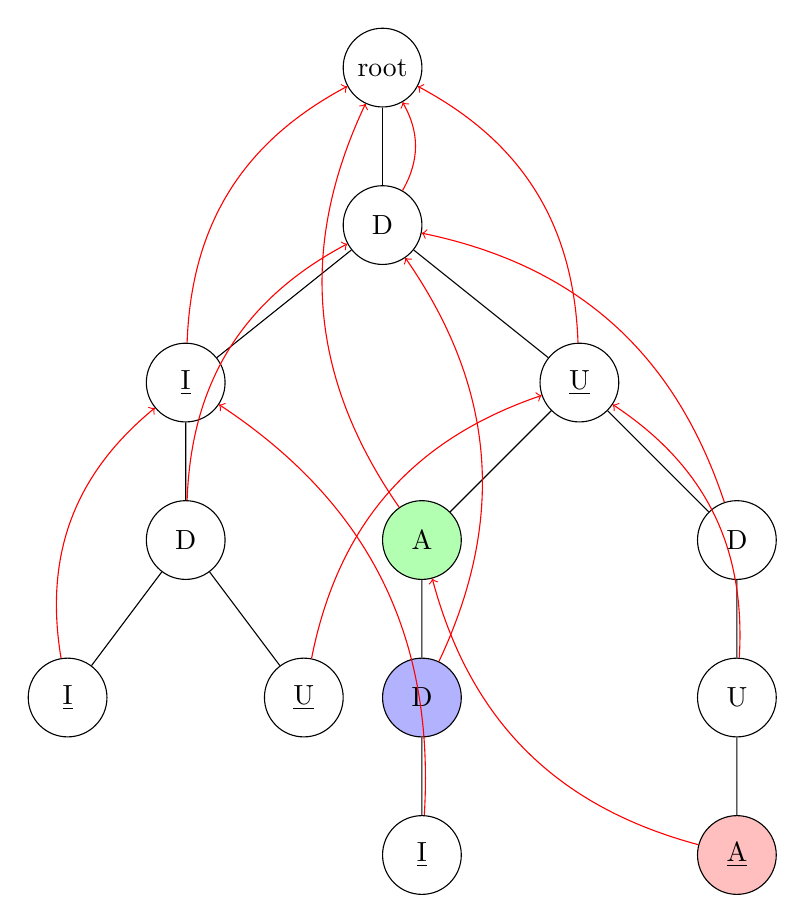
\begin{tikzpicture}[
        level 1/.style={sibling distance=6cm, level distance=2cm},
        level 2/.style={sibling distance=5cm, level distance=2cm},
        level 3/.style={sibling distance=4cm, level distance=2cm},
        level 4/.style={sibling distance=3cm, level distance=2cm},
        level 5/.style={sibling distance=2cm, level distance=2cm},
        level 6/.style={sibling distance=2cm, level distance=2ccm},
        every node/.style={circle, draw, minimum size=1cm}
    ]
        % Vẽ cây chính
        \node (root) {root}
            child { node (D1) {D}
                child { node (I) {\underline{I}}
                    child { node (D2) {D}
                        child { node (I2) {\underline{I}} }
                        child { node (U2) {\underline{U}} }
                    }
                }
                child { node (U1) {\underline{U}}
                    child { node [fill=green!30](A2) {A}
                        child { node [fill=blue!30](D4) {D}
                            child { node (I3) {\underline{I}} }
                        }
                    }
                    child { node (D3) {D}
                        child { node (U3) {U}
                            child { node [fill=pink](A) {\underline{A}} }
                        }
                    }
                }
            };

        % Thêm các liên kết về gốc
        \draw[red, ->] (D1) to[bend right] (root);
        \draw[red, ->] (I) to[bend left] (root);
        \draw[red, ->] (I2) to[bend left] (I);
        \draw[red, ->] (D2) to[bend left] (D1);
        \draw[red, ->] (U1) to[bend right] (root);
        \draw[red, ->] (D3) to[bend right] (D1);
        \draw[red, ->] (U2) to[bend left] (U1);
        \draw[red, ->] (A) to[bend left] (A2);
        \draw[red, ->] (A2) to[bend left] (root);
        \draw[red, ->] (D4) to[bend right] (D1);
        \draw[red, ->] (I3) to[bend right] (I);
        \draw[red, ->] (U3) to[bend right] (U1);
    \end{tikzpicture}

\end{center}
Number of patterns that occur in the text: 4 (DI, DIDU, DU, DUDUA).

Now text[i] = D, but node U doesn't have child node D, we trace back to the node the suffix of node U points at, which is the other node A. The other node A has child node D so we travel to that node D.
\pagebreak

\textbf{Step 10:}
\begin{center}

    \begin{table}[H]
    \centering
    \begin{tabular}{|c|c|c|c|c|c|c|c|c|c|}
    \hline
    pos   &   &   &   &   &   & i &   &   &   \\ \hline
    text  & D & I & D & U & D & U & A & D & I \\ \hline
    \end{tabular}
    \end{table}
    
    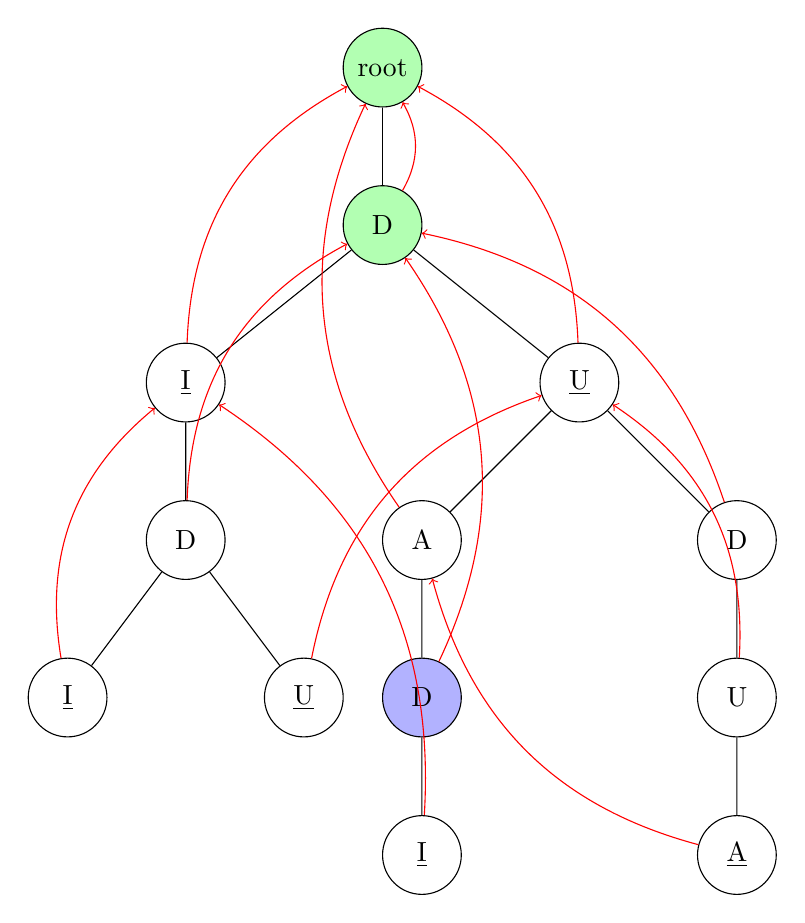
\begin{tikzpicture}[
        level 1/.style={sibling distance=6cm, level distance=2cm},
        level 2/.style={sibling distance=5cm, level distance=2cm},
        level 3/.style={sibling distance=4cm, level distance=2cm},
        level 4/.style={sibling distance=3cm, level distance=2cm},
        level 5/.style={sibling distance=2cm, level distance=2cm},
        level 6/.style={sibling distance=2cm, level distance=2ccm},
        every node/.style={circle, draw, minimum size=1cm}
    ]
        % Vẽ cây chính
        \node [fill=green!30](root) {root}
            child { node [fill=green!30](D1) {D}
                child { node (I) {\underline{I}}
                    child { node (D2) {D}
                        child { node (I2) {\underline{I}} }
                        child { node (U2) {\underline{U}} }
                    }
                }
                child { node (U1) {\underline{U}}
                    child { node (A2) {A}
                        child { node [fill=blue!30](D4) {D}
                            child { node (I3) {\underline{I}} }
                        }
                    }
                    child { node (D3) {D}
                        child { node (U3) {U}
                            child { node (A) {\underline{A}} }
                        }
                    }
                }
            };

        % Thêm các liên kết về gốc
        \draw[red, ->] (D1) to[bend right] (root);
        \draw[red, ->] (I) to[bend left] (root);
        \draw[red, ->] (I2) to[bend left] (I);
        \draw[red, ->] (D2) to[bend left] (D1);
        \draw[red, ->] (U1) to[bend right] (root);
        \draw[red, ->] (D3) to[bend right] (D1);
        \draw[red, ->] (U2) to[bend left] (U1);
        \draw[red, ->] (A) to[bend left] (A2);
        \draw[red, ->] (A2) to[bend left] (root);
        \draw[red, ->] (D4) to[bend right] (D1);
        \draw[red, ->] (I3) to[bend right] (I);
        \draw[red, ->] (U3) to[bend right] (U1);
    \end{tikzpicture}

\end{center}
Number of patterns that occur in the text: 4 (DI, DIDU, DU, DUDUA).

This node D is not the end of ant pattern so we do thing at this node. We trace back to the node the suffix of this node points at, which is the other node D. This node D is also not the end of any pattern so we do nothing at this node. We continue to trace back to the node the suffix of this node points at, which is the root. Because this is the root, we stop the procedure.
\pagebreak

\textbf{Step 11:}
\begin{center}

    \begin{table}[H]
    \centering
    \begin{tabular}{|c|c|c|c|c|c|c|c|c|c|}
    \hline
    pos   &   &   &   &   &   & i &   &   &   \\ \hline
    text  & D & I & D & U & D & U & A & D & I \\ \hline
    \end{tabular}
    \end{table}
    
    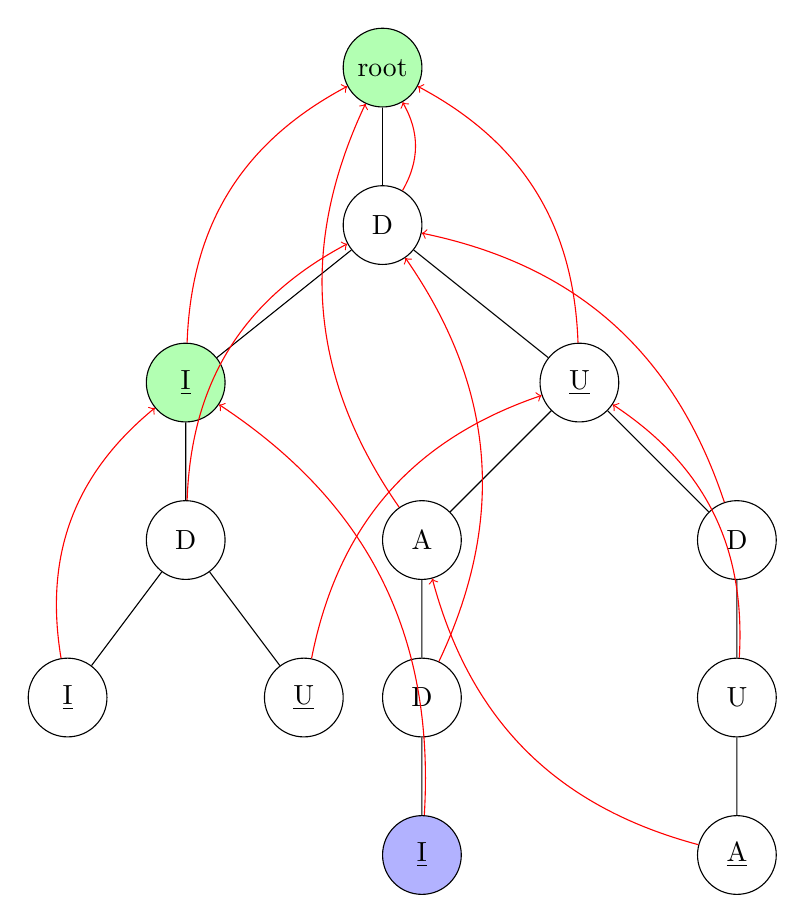
\begin{tikzpicture}[
        level 1/.style={sibling distance=6cm, level distance=2cm},
        level 2/.style={sibling distance=5cm, level distance=2cm},
        level 3/.style={sibling distance=4cm, level distance=2cm},
        level 4/.style={sibling distance=3cm, level distance=2cm},
        level 5/.style={sibling distance=2cm, level distance=2cm},
        level 6/.style={sibling distance=2cm, level distance=2ccm},
        every node/.style={circle, draw, minimum size=1cm}
    ]
        % Vẽ cây chính
        \node [fill=green!30](root) {root}
            child { node (D1) {D}
                child { node [fill=green!30](I) {\underline{I}}
                    child { node (D2) {D}
                        child { node (I2) {\underline{I}} }
                        child { node (U2) {\underline{U}} }
                    }
                }
                child { node (U1) {\underline{U}}
                    child { node (A2) {A}
                        child { node (D4) {D}
                            child { node [fill=blue!30](I3) {\underline{I}} }
                        }
                    }
                    child { node (D3) {D}
                        child { node (U3) {U}
                            child { node (A) {\underline{A}} }
                        }
                    }
                }
            };

        % Thêm các liên kết về gốc
        \draw[red, ->] (D1) to[bend right] (root);
        \draw[red, ->] (I) to[bend left] (root);
        \draw[red, ->] (I2) to[bend left] (I);
        \draw[red, ->] (D2) to[bend left] (D1);
        \draw[red, ->] (U1) to[bend right] (root);
        \draw[red, ->] (D3) to[bend right] (D1);
        \draw[red, ->] (U2) to[bend left] (U1);
        \draw[red, ->] (A) to[bend left] (A2);
        \draw[red, ->] (A2) to[bend left] (root);
        \draw[red, ->] (D4) to[bend right] (D1);
        \draw[red, ->] (I3) to[bend right] (I);
        \draw[red, ->] (U3) to[bend right] (U1);
    \end{tikzpicture}

\end{center}
Number of patterns that occur in the text: 5 (DI, DIDU, DU, DUDUA, DUADI).

Now text[i] = I, we travel to node I from node D. Because this node is the end of pattern DUADI and this pattern have not been counted, the number of patterns that occur in the text is increased by 1. We trace back to the node the suffix link of this node points at, which is other node I. This other node A is the end of pattern DI but this pattern has already been counted so we do nothing on this node. We countinue to trace back to the node the suffix of this node points at, which is the root. Because this is the root, we stop the procedure.
\subsubsection*{Result}
There are 5 patterns occur in the text DIDUDUADI.
\subsection{Complexity Analysis}
\subsubsection*{Trie Construction}
Each pattern is inserted into the trie, where the total length of all patterns is denoted as \( m \). Since inserting each character takes \( O(1) \), the total time complexity of constructing the trie is: \[ O(m) \]

\subsubsection*{Suffix Link Construction}
The suffix links are built using a depth-first search (DFS) traversal  of the trie. Each node and edge is processed once, leading to a complexity of: \[ O(m) \]

\subsubsection*{Text Searching}
Let \( n \) be the length of the text. During the search:

\begin{itemize}
    \item If a transition exists in the trie, we move forward in \( O(1) \).
    \item If there is a mismatch, suffix links guide the search backward.
\end{itemize}

\noindent In the worst case, suffix links may be followed multiple times. However, since each character in the text is processed at most once along with backtracking via suffix links, the total complexity remains: \[O(n + m)\]

\subsubsection*{Best Case}
If the text mostly follows the trie transitions without needing fail links, then each character is processed in \( O(1) \), leading to: \[ O(n) \]

\subsubsection*{Worst Case}
If suffix links are frequently used, a character may trigger multiple backtracking steps. However, across the entire search, the number of such backtracking steps is bounded by \( O(n + m) \). Thus, the worst-case complexity is: \[ O(n + m) \]

\subsubsection*{Conclusion}
The Aho-Corasick algorithm provides an efficient way to search multiple patterns in a text with the following time complexities:

\begin{itemize}
    \item \textbf{Best case:} \( O(n) \), when suffix links are rarely used.
    \item \textbf{Worst case:} \( O(n + m) \), when suffix links cause multiple jumps.
\end{itemize}
\section{Similarities and Dissimilarities Between Aho-Corasick and KMP}
\subsection*{Similarities}
Both Aho-Corasick and Knuth-Morris-Pratt (KMP) are efficient pattern matching algorithms that share the following characteristics:

\begin{enumerate}
    \item \textbf{Preprocessing for Efficient Searching}:  
    Both algorithms preprocess the pattern(s) before searching.
    \item \textbf{Failure Links for Efficient Backtracking}:  
    Both use suffix links to avoid unnecessary comparisons (KMP uses the Longest Prefix Suffix (LPS) array, while AC uses suffix links in a trie).
    \item \textbf{Linear Time Complexity in Searching}:  
    Both achieve an efficient search time of \( O(n) \), where \( n \) is the length of the text.
    \item \textbf{Pattern Matching Without Backtracking}:  
    Neither algorithm requires explicit backtracking in the text; instead, they use precomputed failure information to move efficiently.
\end{enumerate}

\subsection*{Dissimilarities}

\begin{table}[H]
    \centering
    \renewcommand{\arraystretch}{1.3}
    \begin{tabular}{|p{3cm}|p{5cm}|p{5cm}|}
        \hline
        \textbf{Feature} & \textbf{Aho-Corasick (AC)} & \textbf{Knuth-Morris-Pratt (KMP)} \\
        \hline
        \textbf{Purpose} & Searches for multiple patterns simultaneously & Searches for a single pattern \\
        \hline
        \textbf{Preprocessing Complexity} & \( O(M) \), where \( M \) is the total length of all patterns & \( O(m) \), where \( m \) is the length of the pattern \\
        \hline
        \textbf{Search Complexity} & \( O(n + z) \), where \( n \) is the text length and \( z \) is the number of matches & \( O(n) \), where \( n \) is the text length \\
        \hline
        \textbf{Data Structure Used} & Trie with failure (or suffix) links & LPS (Longest Prefix Suffix) array \\
        \hline
        \textbf{Space Complexity} & \( O(M \cdot \sigma) \) in worst-case, where \( \sigma \) is the alphabet size & \( O(m) \) \\
        \hline
        \textbf{Pattern Matching Approach} & Simultaneously matches multiple patterns & Sequentially matches a single pattern \\
        \hline
        \textbf{Common Use Cases} & Spam filtering, intrusion detection, dictionary matching & Substring search in text editors, string matching problems \\
        \hline
    \end{tabular}
    \caption{Comparison of Aho-Corasick and KMP Algorithms \texttt{[H]}}
    \label{tab:dissimilarities}
\end{table}

\subsection*{Conclusion}
\begin{itemize}
    \item \textbf{Aho-Corasick} is preferable when searching for multiple patterns at the same time.
    \item \textbf{KMP} is more suitable for efficiently searching a single pattern in a text.
\end{itemize}




\section{Team Progress}
\hspace*{-3.5cm}
\begin{longtable}{|c|>{\raggedright\arraybackslash}p{2.8cm}|>{\centering\arraybackslash}p{8cm}|c|c|}
\hline
\textbf{No.} & \textbf{Member Name} & \textbf{Assigned Tasks} & \textbf{Completion} & \textbf{Timeline} \\
\hline
1 & Trịnh Duy Nhân &
\raggedright
- Analyze and identify the Aho-Corasick algorithm \newline
- Preprocess multiple patterns using Trie data structure \newline
- Perform string matching \newline
- Write report sections 4 and 5 \newline
- Create PowerPoint slides &
100\% & 12/03 – 03/04 \\
\cline{3-5}
& &
\raggedright
- Present the preprocessing and matching process of the Aho-Corasick algorithm, followed by a comparison of similarities and differences between the two algorithms &
100\% & 05/04 \\
\hline
2 & Võ Đình Cao Minh Hào &
\raggedright
- Analyze and identify the KMP algorithm \newline
- Preprocess strings using Trie \newline
- Perform string matching \newline
- Write report sections 2 and 6 \newline
- Create PowerPoint slides &
100\% & 12/03 – 03/04 \\
\cline{3-5}
& &
\raggedright
- Present the preprocessing and string matching process of the KMP algorithm &
100\% & 05/04 \\
\hline
3 & Phan Thanh Trúc Quân &
\raggedright
- Write report sections 1, 3, and 7 &
100\% & 12/03 – 03/04 \\
\cline{3-5}
& &
\raggedright
- Present the definition, problem, and main idea of both KMP and Aho-Corasick algorithms &
100\% & 05/04 \\
\hline
\end{longtable}


\section{Presentation Video}
\href{https://drive.google.com/file/d/1YZvHunws_VdB13_Il37dTGiP3yG2GYvu/view?usp=sharing}{Click here} to watch the video
\cleardoublepage
\phantomsection
\addcontentsline{toc}{section}{References}
\bibliographystyle{plain}
\bibliography{ref/ref}
\end{document}



